%% ----------------------------------------------------------------
%% Thesis.tex -- MAIN FILE (the one that you compile with LaTeX)
%% ----------------------------------------------------------------

% Set up the document
\documentclass[a4paper, 11pt, oneside]{Thesis}  % Use the "Thesis" style, based on the ECS Thesis style by Steve Gunn
\graphicspath{{Figures/}}  % Location of the graphics files (set up for graphics to be in PDF format)

% Include any extra LaTeX packages required
\usepackage[square, numbers, comma, sort&compress]{natbib}  % Use the "Natbib" style for the references in the Bibliography
\usepackage[english, hungarian]{babel}
\usepackage[utf8]{inputenc}
\usepackage[T1]{fontenc}
\usepackage{verbatim}  % Needed for the "comment" environment to make LaTeX comments
\usepackage{vector}  % Allows "\bvec{}" and "\buvec{}" for
                     % "blackboard" style bold vectors in maths
\usepackage{xr}
\usepackage{hyperref}
\usepackage[table]{xcolor}
\usepackage{multirow}
\usepackage{array,booktabs}
\hypersetup{urlcolor=blue, colorlinks=true}  % Colours hyperlinks in blue, but this can be distracting if there are many links.

%%Renewing some commands so they don't appear in Hungarian
%%names gotten from: %%/usr/share/texmf-texlive/tex/generic/babel/magyar.ldf
%%modified line 111 there to change how the figure name is displayed

\addto\captionshungarian{%
  \renewcommand{\listfigurename}%
    {List of Figures}%
}

\addto\captionshungarian{%
  \renewcommand{\listtablename}%
    {List of Tables}%
}

\addto\captionshungarian{%
  \renewcommand{\bibname}%
    {Bibliography}%
}

\addto\captionshungarian{%
  \renewcommand{\contentsname}%
    {Contents}%
}

\addto\captionshungarian{%
  \renewcommand{\figurename}%
    {Figure}%
}

\addto\captionshungarian{%
  \renewcommand{\chaptername}%
    {Chapter}%
}

\addto\captionshungarian{%
  \renewcommand{\tablename}%
    {Table}%
}

\newcommand{\methodname}[1] {
\\[0.2cm]
\ttfamily #1\normalfont
}

%% ----------------------------------------------------------------
\begin{document}
\frontmatter      % Begin Roman style (i, ii, iii, iv...) page numbering

% Set up the Title Page
\title  {A testing framework and workflow for validation and
  improvement of the SMPI simulation framework for MPI applications}
\authors  {\texorpdfstring
            {\href{your web site or email address}{Attila Döme Lehóczky}}
            {Attila Döme Lehóczky}
            }
\addresses  {\groupname\\\deptname\\\univname}  % Do not change this here, instead these must be set in the "Thesis.cls" file, please look through it instead
\date       {\today}
\subject    {}
\keywords   {}

\maketitle
%% ----------------------------------------------------------------

\setstretch{1.3}  % It is better to have smaller font and larger line spacing than the other way round

% Define the page headers using the FancyHdr package and set up for one-sided printing
\fancyhead{}  % Clears all page headers and footers
\rhead{\thepage}  % Sets the right side header to show the page number
\lhead{}  % Clears the left side page header

%% ----------------------------------------------------------------
% The "Funny Quote Page"
\pagestyle{empty}  % No headers or footers for the following pages

\null\vfill
% Now comes the "Funny Quote", written in italics
\textit{``Groovy!''}

\begin{flushright}
%If the quote is taken from someone, their name goes here
\end{flushright}

\vfill\vfill\vfill\vfill\vfill\vfill\null
\clearpage  % Funny Quote page ended, start a new page
%% ----------------------------------------------------------------

% The Abstract Page
\addtotoc{Abstract}  % Add the "Abstract" page entry to the Contents
\abstract{
\addtocontents{toc}{\vspace{1em}}  % Add a gap in the Contents, for aesthetics

SimGrid is a generic simulation framework, which can be used to
simulate multiple kinds of distributed systems, such as
Clouds, Grids or clusters. SMPI is a framework that connects SimGrid
with the MPI inter-process communication protocol: it's part of the
SimGrid project with the goal of running MPI applications in a
simulated environment. SMPI is currently under heavy development, thus
in need of constant validation. This thesis is about the
implementation of a framework that could help in orchestrating and
automatizing tests with the goal of aiding the development of the
project. SMPI validation is done by
running real-life MPI benchmarks (using possibly multiple different
implementations), as well as running the same benchmarks with
SMPI. The results can be used to check how accurate the simulation
was. Currently, this testing process consists of multiple
manually performed steps. It's tedious, repetitive work, but as
mentioned before, it's necessary. The main goal of the framework is to
provide a means to orchestrate such tests, introducing as much
automation into the process as possible, providing the possibility to
create test workflows that could be run with minimal user
interaction. With that, we could provide the possibility to speed up
the testing process, making it possible to acquire proportionally more
test results, thus helping the development team to make progress.
}
\clearpage  % Abstract ended, start a new page
%% ----------------------------------------------------------------

\setstretch{1.3}  % Reset the line-spacing to 1.3 for body text (if it has changed)

% The Acknowledgements page, for thanking everyone
\acknowledgements{
\addtocontents{toc}{\vspace{1em}}  % Add a gap in the Contents, for aesthetics

The author would like to thank his supervisor, Mark Stillwell for
the opportunity to write this thesis, as well as for his counsel and
guidance throughout the project. The author would also like to
extend his thanks to George Markomanolis and Tomasz Buchert for
providing invaluable advice and selfless support when it was needed
the most.\\[0.5cm]
Last but not least, the author wants to give a very special thanks
to his family and his fiancée for their never-ending love and
support. Without them, this thesis wouldn't have been possible to
make.

}
\clearpage  % End of the Acknowledgements
%% ----------------------------------------------------------------

\pagestyle{fancy}  %The page style headers have been "empty" all this time, now use the "fancy" headers as defined before to bring them back


%% ----------------------------------------------------------------
\lhead{\emph{Contents}}  % Set the left side page header to "Contents"
\tableofcontents  % Write out the Table of Contents

%% ----------------------------------------------------------------
\lhead{\emph{List of Figures}}  % Set the left side page header to "List if Figures"
\listoffigures  % Write out the List of Figures

%% ----------------------------------------------------------------
\lhead{\emph{List of Tables}}  % Set the left side page header to "List of Tables"
\listoftables  % Write out the List of Tables

%% ----------------------------------------------------------------
\setstretch{1.3}  % Return the line spacing back to 1.3

%% ----------------------------------------------------------------
\mainmatter   % Begin normal, numeric (1,2,3...) page numbering
\pagestyle{fancy}  % Return the page headers back to the "fancy" style

% Include the chapters of the thesis, as separate files
% Just uncomment the lines as you write the chapters

% Chapter 1

\chapter{Chapter Title Here} % Write in your own chapter title
\label{Chapter1}
\lhead{Chapter 1. \emph{Chapter Title}} % Write in your own chapter title to set the page header

\section{Welcome and Thank You}

\subsection{Examples of \LaTeX{} Typeset eBooks}

\section{Learning \LaTeX{}}

\subsection{A (not so short) Introduction to \LaTeX{}}

\subsection{A Short Math Guide for \LaTeX{}}
\section{The `\texttt{Thesis.tex}' File Explained}

 % Introduction

% Chapter 2

\chapter{Literature Review}
\label{Chapter2}
\lhead{Chapter 2. \emph{Literature Review}}

In the literature review, we discuss the area of research covered by
the thesis, citing relevant papers and articles that serve as a base
of ideas for this document.\\
First, we talk about the Message-Passing Interface (MPI), the parallel
programming API used for the purposes of this thesis. We also talk
about the different implementations of this API, notably OpenMPI and
MPICH. We discuss the methods of modelling and simulation in general.
Then, we talk about SimGrid, which is a simulation-based
framework, and SMPI, the implementation of MPI that runs on top of
SimGrid. While discussing SMPI, we present the idea of a framework
that would make it possible to automate running tests, trace
collection and post-processing. In connection to this framework, we
talk about workflows as a means to automate our experiments and
whether scientific or business workflows are more suitable for
us. We also talk about the importance of reproducible research, which
is another argument for constructing such a framework.
\section{MPI}
Distributed computing is a very active and important subject of research
in computer science, including fields such as cluster computing, grid
computing, Cloud computing, or peer-to-peer computing. Communication
between the different processes in a distributed application can be
implemented in a number of ways. As communication is necessary in most
cases, a standardized communication protocol can be a lot of help when
developing a distributed program. The Message-Passing Interface (MPI)
is a language-independent message-passing library
interface specification. It is not a language, but a standard - there
exist multiple MPI implementations. Since its take-off, it has become
a de facto standard for inter-process communication. The standard
provides vendors a clear set of routines, that they can implement
efficiently, or in a way that it suits the hardware they
provide.\cite{mpif12}
\subsection{OpenMPI}
OpenMPI is an MPI implementation with the goal of being able to
achieve good performance on a wide range of different aspects of
high-performance computing. To efficiently support multiple types of
parallel machines, high performance “drivers” for all established
interconnects are developed. These include TCP/IP, shared memory,
Myrinet, Quadrics, and Infiniband. Features for checking data
integrity are provided in order to account for network transmission
errors. With the utilization of message fragmentation and striping
over multiple (potentially heterogeneous) network devices, OpenMPI
provides an increased bandwidth to applications, as well as the
ability to handle the failure of network devices during
runtime.\cite{ompi04} On the Grid'5000 cluster, which is used to most
of the research conducted for this thesis, OpenMPI is the default MPI
implementation used by the default images.
\subsection{MPICH}
MPICH was originally developed during the MPI standards process
starting in 1992 to provide feedback to the MPI Forum on
implementation and usability issues. This original implementation was
based on the Chameleon portability system to provide a light-weight
implementation layer (hence the name MPICH from MPI over
CHameleon). Around August 2001, development begun on a new
implementation called MPICH2.\cite{mpich12} This implementation
introduced improvements on collective communication operations by
using multiple algorithms, choosing between them depending on certain
variables - for example the message size.\cite{trg05} Another
important result during the development of MPICH2 was the design of
the Nemesis communication subsystem and the porting of MPICH2 on that
system. The efficient implementation of shared-memory communication
helped Nemesis MPICH2 achieve low latency and high
bandwidth.\cite{bmg07}\\
Starting with November 2012, the project is renamed to MPICH, with
version number 3.0.\cite{mpich12}
\section{Modelling and Simulation}
In distributed computing, modelling means creating an abstraction of a
real system by taking only the aspects of it that are relevant to the
system's behavior into account. Once constructed, such a model becomes
a tool with which we can investigate the behavior of the
system.\cite{h12_1}
\subsection{Advantages of Modelling}
Modelling and simulation techniques have been used extensively in
parallel computing and is an ongoing research topic, with new
challenges continuously arising. There are various reasons for its
importance.\\
Conducting experiments on real-world systems can be
infeasible because experimenting would disrupt the service that is
provided by the system. For example, in the case of a mail server,
experiments or monitoring could cause delay, or maybe even data
loss. Service disruption can sometimes be even dangerous, in addition
to being an inconvenience: in the case of a nuclear reactor, delay or
loss of data can prove fatal. Timeliness can be as important in such
systems as correctness. However, performance analysis and monitoring
might be crucial to draw conclusions about maintenance, for
example. Another problem with direct experimentation is that the
information we are looking for may not be available, or may be
complicated to get. For example, in most operating systems, it is
difficult to obtain the exact timing of instruction-level
events.\cite{h12_1} Also, when conducting experiments on a real-world
system, results are often non-reproducible, due to resource
dynamics.\cite{clq08} Another argument on the side of modelling is
that it provides the ability of experimenting on different
configurations. Investing in a large-scale computer cluster, or the
setup of a distributed grid environment is an expensive and tedious
process. Investors want to make sure that they get what they
want: they impose performance constraints on the system. This means
that they want to know how the system will behave
before buying it and setting it up. To predict the behavior,
experiments are needed to be conducted. We need to do these
experiments on different setups, before finding out which one is the
best in the current situation. Changing the hardware or software
configuration parameters on a real-world system is very inconvenient -
in most cases, it's not doable, because of time and money
constraints. Thus, the solution is to simulate the desired
system, and run the experiments there. This way, changing the
configuration is simple and costless.\cite{h12_1} Another great
benefit of simulation is that in a classroom setting, students can
learn the principles of high-performance and distributed computing
without actual access to a parallel platform.\cite{csgscq11}
\subsection{Analytical and Simulation Models}
The accuracy of a model can vary: we can make an analytical, or
qualitative model, in which all definite values are abstracted away -
in this case, we get a representation of
the system, which can be analysed mathematically to deduce its
behavior. When using this method, no experiments can be conducted, we
solely rely on theoretical analysis. In contrast, a simulation model
is a stochastic model, which is an algorithmic abstraction of the
real-world system that can be executed to reproduce the system's
behavior. This model is also called a quantitative model, as we can
get estimates of the modeled system's quantitative attributes, such as
response time or throughput. In other words, we can use a simulation
model to conduct performance analysis on a system, without actually
having the actual system at our disposal.\cite{h12_1}\cite{h12_13}\\
When wanting to get a prediction about how a specific system would
perform, a theoretical model, in most cases, produces unreliable and
unrealistic results - it's not feasible for such accurate
predictions. The vast majority of research results are obtained via
empirical evaluation of experiments.\cite{clq08} For these reasons, we
use the simulation model in this thesis. As we stated before, such a
model can be executed, which is called simulation. During simulation,
the model is supposed to behave like the real system would. It is hard
to produce a 100\% accurate simulation, but more and more reliable
solutions are being developed. The simulation model contains
more aspects of the real system compared to the theoretical model, in
order to accurately represent the system, while still avoiding
unnecessary detail.\cite{h12_1} Creating and executing a simulation
model is complicated, computationally expensive and poses a number of
challenges, thus, a good simulation framework (such as SMPI) can prove
to be of much help when conducting experiments.
\section{Off-line and partial on-line simulation}
Full simulation - including CPU and network emulation - of a parallel
application can be, in many cases, even more resource-intensive than
running real-world experiments. This contradicts the fact that one of
the most prominent goals of simulation is to observe the behavior of
such large-scale platforms that aren't available. Thus, there is much
interest in more efficient simulation approaches. \cite{bdglmqssv13}
The most widely used of such approaches fall into two categories:
off-line simulation, which is also called trace-based or post-mortem
simulation and on-line simulation, which is simulation via direct
execution.\cite{csgscq11} As in the subject of this thesis, we are
interested only in the simulation of MPI applications, we describe
the two different simulation approaches concentrating specifically on
that subject.
\subsection{Off-line simulation}
For conducting off-line simulation, logs or traces are needed to be
collected of an execution of the MPI application to be simulated,
taking place on a
real-world platform. This is necessary because the obtained traces are
used as an input for the simulator, which then replays the execution
traces as if the application was running on the target platform. This
platform's characteristics may differ from the one's that we obtained
the traces from, since we may want to use the simulator to predict the
application's performance on a different system. Thus, there is a need
to calculate how the target platform would execute the application,
based on the traces we got on the other platform. The typical approach
to this problem is to first compute the time intervals between the MPI
communication operations. During these intervals, local computations
were conducted, that's why we call these "CPU bursts". During
simulation, we have to account for the differences between the
performance of the platforms by modifying the time these CPU bursts
take. This can be done by simply scaling the time intervals, or by
using more sophisticated methods, by calculating exactly how the
application's computational signature and the platform's hardware
signature relate.\cite{csgscq11} Communication operations, of course,
also need to be simulated. This is done based on the events recorded
on the trace, and on the network model of the simulated
platform.\cite{csgscq11}\\
As mentioned in \cite{csgscq11}, there are multiple downsides and
challenges to the off-line approach. On such downside is that when
wanting to simulate a relatively larger-scale application, the size of
the obtained traces can be so large, that running the simulation on a
single node might become a problem. Methods in order to overcome this
obstacle include a compact representation of the traces in order to
reduce its size. Another solution is to only consider a carefully
selected subset of the obtained traces. A big disadvantage when using
off-line simulation is that because we use the traces as an input to
the simulator in order to replay the execution of the application, the
simulation is dependant on the platform we collect the traces
on. This means that, for example, there can be features in the
obtained traces that might not be available on the target platform. In
most cases, it is also necessary that the two platforms have the same
number of nodes to run the experiment on. Although there has been a
good amount of research done in the area, MPI itself and also the
application might alter its behavior depending on problem and message
size. Because of this, simulating the scaling of an application is a
very hard, if not impossible task.\cite{bdglmqssv13}
\subsubsection{Time-independent traces}
Another link that ties the produced trace to the host platform occurs
when we use timed traces, meaning that each traced event is associated
to a time-stamp. Since the time delays between the events are specific
to the platform specification, the simulator has to apply a correction
factor to these delays when running the simulation on the target
platform. Thus, the simulator has to know precisely the specification
of both the host and the target platform, in order to be able to
calculate this correction factor. Another difficulty regarding that
comes up regarding this problem is that actually calculating the
correction factor is a tedious process. It can take a considerable
amount of time, depending on how similar the host and the target
platforms are.\cite{dmsq11}\\
In \cite{dmsq11}, a solution to this problem is proposed:
time-independent traces. Acquiring time-independent traces means that
the traces won't contain any timestamps, breaking this link between
the acquisition and the replay of the traces. In these type of traces,
for each computation or communication operation, we log the volume of
the operation (in number of floating point operations or bytes)
instead of the time the execution took. This type of information, in
most cases, does not vary depending on the platform the experiment is
run on. The exceptions are the adaptive MPI applications that modify
their execution path according to the execution platform.\\
\cite{ms11} contains a guide describing how to acquire such traces on
the Grid5000 platform. The guide was used to serve as a base for the
process on how to acquire traces. Since the work in this thesis is
mostly related to producing traces for validating on-line simulation,
in which case time-stamps don't have an influence on the process
(neither in a positive, nor a negative way), the extraction of
time-independent information from the traces can be omitted in our
case.
\subsection{Partial on-line simulation}
Partial on-line simulation is a different approach. Here, we execute
the program with no or very little modification on a host platform,
that tries to mimic the behavior of the target
platform.\cite{csgscq11} Computational tasks are executed on the
hardware, but the timing and the delivery of the messages is
calculated by the simulation environment. Thus, the simulator is
responsible for mainaining the correct order of the events, both
computational and communicational.\cite{bdglmqssv13}\\
A downside of the on-line approach is that since we actually execute
the code, the resource needs for running the simulation is about as
high or even higher (in case of needing an extra node to run the
simulation component, for example) than it is for the actual
experiment. Techniques have been implemented in order to help
alleviate this problem. The basic idea is that
the actual results of the experiments (for example, the result of
multiplying two matrices) might not be important in our case: we are
only interested in the \emph{time} it takes to get those results on
the target platform. This is why methods can be employed which trade
off accuracy for performance. This idea might not be feasible for
experiments where data-dependent application behavior is
vital, but a large portion of benchmarks can be indeed simulated
this way, providing a reasonably accurate execution profile.\\
Although slower, on-line simulation is more general than the off-line
approach, as it does not, in any way depend on some other platform -
whereas in the case of off-line simulation, as we mentioned before,
the trace is acquired on a different platform, with maybe specific
application configurations, thus inevitably bringing dependencies.
\section{SimGrid}
For reasons mentioned before, simulation techniques have historically
been widely utilised in several areas of computer science,
e.g. microprocessor design, network protocol design. Due to this, a
lot of effort went into developing the technology and as a result,
widely used and reliable simulation frameworks have been developed in
these areas. However, there hasn't been a well-developed standard
simulation tool for what we talk about in this thesis: execution of
distributed applications on distributed computing platforms. Rather,
there has only been a number of in-house developed, highly specialized
tools to satisfy the need of the community. SimGrid is a more generic
simulation framework that is being developed to be one of the
acknowledged and widespread tools for simulation in large-scale
distributed computing.\cite{clq08}\\
SimGrid's key features include:\cite{clq08}
\begin{itemize}
\item A scalable and extensible simulation engine that implements
  several validated simulation models, and that makes it possible to
  simulate arbitrary network topologies, dynamic computational and
  network resource availabilities, as well as resource failures;
\item High-level user interfaces for researchers (who are not
  necessarily computer science experts, but rather experts on their own
  field of research) to quickly assemble simulation prototypes in either
  C or Java;
\item APIs for distributed computing developers to create distributed
  applications that can run seamlessly in either "simulation mode" or
  "real-world mode", in order to be able to test it on the simulated
  environment before actually deploying it.
\end{itemize}
SimGrid is a very active project, both in terms of research and in
terms of development. It is a favored tool by researchers, which is
proven by the increasing number of papers written where the research
was conducted using SimGrid as a scientific instrument. In terms of
development, the developer team envisions a number of directions for
future work: addition of a model for disk resources; extention of
scalability to improve usability in the P2P domain; ability to
dispatch simulated nodes over several physical machines.\cite{clq08}
Another important field of research for the SimGrid team is the
implementation of the API that has already been mentioned: the
Message-Passing Interface (MPI).
\section{SMPI}
As stated before, MPI is one of the most widely used APIs for
communication between nodes in distributed computing. SMPI is a
framework for simulating on a single node the execution of parallel
applications implemented using the MPI standard. It is part of the
SimGrid project and as such, it is built on the SimGrid simulation
kernel, benefiting from its fast, scalable and validated network
models. SMPI also extends the existing model with other techniques,
such as a validated piece-wise linear model for data transfer times
between cluster nodes. SMPI simulations also account for network
contention - timing and delivery of the messages are determined using
the network model of SimGrid.\cite{csgscq11} A current limitation in
SMPI is that it is unable to simulate high-performance networking
hardware such as Infiniband. Thus, when wanting to compare simulation
to real-life results, we have to make sure those results were gatheres
using Gigabit ethernet.\\
Three of the main challenges for simulating an MPI application are:
\begin{itemize}
\item Accuracy: The prediction of the real-world execution time (the
  "simulated time") needs to be as accurate as possible, so that
  reasonable conclusions can be drawn from the experiments.
\item Scalability: We want to be able to simulate large-scale
  applications within a reasonable timescale.
\item Speed: It would be advantageous if the simulation time (the
  actual time of running the simulation) would be as low as possible,
  compared to the simulated time (the predicted execution time of the
  real-world application).
\end{itemize}
As for simulation methods, SMPI can be used for both off-line and
on-line simulation, although the emphasis is more on the on-line
approach, since it's actually a partial implementation of the MPI
standard in itself, thus making it feasible for executing MPI
experiments. More specifically, in SMPI, the goal is to be able to
make such simulations on a single node. The most prominent challenges
when doing this are the large CPU and memory requirements. SMPI
provides some special techniques that help overcoming these
challenges. The basic idea about trading off accuracy for performance
has already been described in the previous section about on-line
simulation. SMPI implements multiple such techniques, allowing to run
experiments with such high resource requirements that would otherwise
be impossible to fulfill. Such a method in order to reduce CPU usage
is to run the
benchmark only on a subset of all the nodes, while in place of running
the code on the others as well, we just insert the computation time
that we got previously. Apart from CPU usage, we need to also account
for the need for memory. A technique for that is "RAM folding": here,
multiple simulated processes, that in SMPI are, in fact, simple
threads, use the same reserved memory location, thus overwriting each
other's data structures. Also, another implemented solution is to
remove large data array references from the code, with the help of the
compiler which can result in the complete removal of potentially
large, now unreferenced arrays. Again, this obviously corrupts the
results that the experiment program gives, but in the same time helps
to simulate applications that would use such an amount of memory that
just wouldn't be physically possible to provide in our testing
environment, while still providing a reliable estimate of the
performance.\cite{bdglmqssv13} These features are disabled by default,
they have to be explicitly enabled by the user.\\
Extensive testing was conducted in \cite{csgscq11} to verify the
previously mentioned qualities of the framework. In these tests, the
OpenMPI and MPICH implementations were used to serve as verification
benchmarks: the same experiments were run using both MPI
implementations, as well as simulated with SMPI. The
results show that SMPI predicted the execution time of OpenMPI and
MPICH applications for point-to-point, one-to-many and many-to-many
applications with an average error value of under 10\% in each
cases. Using the aforementioned techniques to reduce the memory
footprint, SMPI tests
were successfully conducted on a scale of up to 448 processors. The
results showed that the predicted execution times were
underestimates with an average error value of 18.5\%, which is higher
than in previous experiments without these techniques. We have to note
here, though, that
certain tests weren't successful without the RAM-folding techniques,
due to an out-of-memory error. This shows, that although it poses
difficulties, reducing the memory usage is vital in SMPI.\\
As SMPI is an actively developed project alongside SimGrid, there are
a number of research directions. One major development to the
project would be a testing framework that would aim to lessen the
burdens of testing as much as possible. The goal is to provide a
unified method to set up experiments across different environments and
to do it with as little necessary adjustments on user part as
possible.
\section{Experimentation tools}
Experiment orchestration and process automation is not a new
idea. There exist multiple tools for doing this. Among others, such
tools are Expo\cite{vr08}, Plush, OMF\cite{rosj09} or the
Grid5000-specific g5k-campaign. The problem is that most of these
tools use a bottom-up design, meaning that in order to understand and
use the experiments, the user has to understand the lower-level
building blocks first. A top-down approach would make it possible to
start the design of the experiment with a high-level description, then
work our way down to the lower level details while implementing. There
already exists an approach like this, in Business Process
Management (BPM).\cite{bn12_2} Before talking about BPM though, let's
take a glance at workflows in general.
\section{Workflows}
When talking about a framework to automate MPI experiments, we are
essentially talking about creating workflows: we connect multiple
steps, making it possible to execute them in a chain, with no or
minimal user interaction during the process. In the application level,
workflows are abstract in the sense that the workflow only describes
the goal of the experiment, its components and its dependencies. Lower
level implementation details are hidden from the user of the
workflow. This provides the possibility of changing the implementation
without having to change the high-level workflow description - as long
as the new implementation still has the properties that are written in
the description.\cite{dssbgkmvbgljk05}
In the subject of workflows, there are two main approaches that we
will discuss: scientific workflows and the previously mentioned
business workflows.
\subsection{Scientific workflows}
Scientific analyses often have to be conducted in several different
hardware and software environments. Exporting and importing data from
and to different environments can be a tedious task, slowing down the
work process, forcing researchers to divide their efforts between
computation management and their actual research. This is the main
reason scientific workflows are widely used in various different
scientific domains: they are a formalization of the ad-hoc
process that a scientist has to go through in order to get from raw
data to publishable results. Since the raw data to be analyzed can be
large, heterogeneous and complex, the process can be computationally
intensive and produce derived data formats, which is one of the main
differences between scientific and business
workflows.\cite{abjjlm04}\\
There are several tools that help in experiment design, mapping of
computing resources to the workflow and handling exceptional
situations. Some of the more well-known tools include
Kepler\cite{abjjlm04}, Pegasus\cite{dssbgkmvbgljk05} and
Taverna\cite{whfwwsdnfbbbhnvsg13}.\\
Scientific workflows are well suited for managing computation on
\emph{a priori} available data or data queried from public
databases. However, it's not well suited to cases when data
acquisition is actually part of the workflow process, or in other
words, when the source of the data is the computer system
itself. They are also data flow-driven, which is not true in the case
of our processes that we want to automate. This makes scientific
workflows not optimal for research conducted in computer science.
\subsection{Business workflows}
Business workflow management systems are usually based on agreed-upon
standards in order to facilitate communication between different
software systems and companies. The workflow logic is control
flow-driven and includes constructs to specify paths and
conditions.\cite{skd10} The top-down approach it uses is what can make
it viable in our case: in Business Process Management, the first step
is to understand the organization. Then we can model its processes as
workflows and execute and monitor them. While monitoring,
we can spot defects and work out ways to improve the organizational
activities, as well as we can redesign the processes to make them
cheaper and faster.\cite{bn12_2}\\
This approach can be utilized in the domain of experiment
orchestration, making business workflows a viable choice when
approaching our problem. An experimentation engine with the goal of
implementing this idea is XPflow\cite{bn12_2}. This engine was used to
implement the test automation framework in this thesis and will be
discussed in a bit more detail later on in this document.
\section{Reproducible research}
New scientific ideas, developments and results are only useful when
they are documented and published. It is vital that results are
announced, so others can be aware of the latest developments on their
field of research. This helps in creating a linked data cloud, used by
scientists to incorporate various output of other research into their
own, using previous results as "stepping stones" to achieve something
new.\cite{babbccrddg10} But simply publishing results is not enough in
order for others to make use of them. Besides announcing the
achievements, the other goal of scientific publications is to convince
the readers that the results it presents are correct. Besides
theoretical reasoning, papers in experimental science should provide a
documented methodology describing how the author has gotten to those
results.\cite{m10} The methodology has to be detailed and precise
enough so other researchers can repeat the same steps, thus
reproducing the same results. This is vital in order to provide the
possibility to verify those results and to fully understand
them. We have to note that in a reproduced experiment, it's not the
\emph{raw results} that need to be identical: they merely need to fit
within a statistical margin, compared to the original results, so that
the \emph{conclusions} derived from them can be the same.\\
Reproducing the results also makes for a starting point for
further development, as the described methods used for reproduction
can be extended to achieve something more or something different in
the same area of research, or repurposed to gain useful results in a
completely different area. Reproducibility is a relevant concern in
the case of SMPI and one of the main goals of the testing and
validation framework is to make developments in the area.\\[0.5cm]
In this chapter, we reviewed the background material to the general
concepts related to this thesis. We talked about the MPI inter-process
communication API and its two different implementations: OpenMPI and
MPICH. Then we talked about modeling and simulation in general and how
simulation is advantageous in certain situations. Relating to
simulation, we talked about SimGrid, a multi-purpose simulation
framework. Then we talked about the project that interconnects these
concepts: SMPI, which is a tool that is able to simulate MPI programs
on SimGrid. We talked about its features and how it's been previously
validated with extensive testing. Since testing is currently a tedious
multi-step process and continuous validation is necessary, the project
is in need of a test automation framework to help with the development
process. Also, such a framework would make documented experiments
repeatable, as well as the results reproducible, which is an important
concern as well. The subject of this framework is connected to the
subject of workflows, which we discussed in some detail in the section
after. We discussed workflows in general, as well as scientific and
business workflows. We concluded that business workflows are more
suitable for our current problem because of its top-down, control
flow-driven approach. We briefly mentioned the XPflow experimentation
engine, which is based on this approach and is utilized in
implementing the framework. In the end, we also discussed the
importance of reproducible research, which is another important aspect
in our motivation for wanting to create the automation framework.
 % Literature Review

% Chapter 3

\chapter{Problem Description}
\label{Chapter3}
\lhead{Chapter 3. \emph{Problem Description}}

In this chapter, we approach the problem regarding the creation of our
framework from different aspects. First, we describe the most
important attributes we'd like the framework to have. After that, we
talk about how trace collection is done, elaborating on the current
manual process of obtaining real-life (RL) traces, illustrating why
it's repetitive error-prone, thus emphasizing the need of
automation. After that, we shed light on some obstacles regarding
tracing, such as tracing overhead or clock synchronization
problems. While discussing these, we also mention some possible ways
of overcoming these obstacles.
\section{Testing framework}
As we previously discussed, there are two main reasons why a test
automation framework is needed by the SMPI project. It's a fact that
the current process is undocumented, long, repetitive and
error-prone. Thus,
\begin{itemize}
\item the heavy development that is currently ongoing in the SMPI
  project is impeded, since development brings with it a constant need
  for validation, which is done by running test.
\item The effort required to reproduce research results related to
  SMPI are needed to be minimized.
\end{itemize}
When specifying the framework, we need to lay down a certain
set of desired properties that we want it to have. The
following is a brief description of these properties, relying on some
of the ideas in \cite{bn12_1}. Some of these attributes will be
elaborated on in greater detail later on in this document.
\paragraph{Scalability}
We want to create experiments with this framework where if we increase
the amount of resources (for example, we run the experiment on more
nodes), then there is no unnecessarily drastic increase in the
preparation or the execution time, the results remain correct and the
execution is free of failures. The unavoidable errors need to be
handled accordingly, providing the user with the necessary details of
what went wrong.
\paragraph{Descriptiveness}
We want to describe our experiments in a top-down approach. This means
that first, we describe the meaning of the experiment: what its goal
is. The lower-level details (how the experiment is conducted, what
tools we use, etc.) are also provided, but they are not necessary to
understand the purpose of the experiment. Providing the possibility to
ignore the details helps to quickly understand the different
experiments, even for newcomers.
\paragraph{Modularity}
We want our experiments to be built from independent, interchangeable
"building blocks". This way, existing experiments can be used as a
starting point: certain parts can be modified, while others can be
left in place, creating a workflow that achieves something
different. Also, modularity helps maintaining the framework: the
different parts can be modified, improved, or even completely
rewritten, not affecting the other modules in the tool.
\paragraph{Reusability}
This attribute intertwines with \emph{modularity} in the sense that we
want to be able to reuse certain parts of the experiments when
creating new ones. This not just eases the work of others in the
research group, but also provides any researcher the possibility to
reuse already written code, so they can reproduce our results or
modify the code to alter the behavior of the workflow.
\paragraph{Error handling}
As mentioned in \emph{scalability}, there are unavoidable errors that
happen from time to time: network issues, unreachable nodes,
deployment failure, etc. Such errors need to be handled gracefully:
the program needs to provide information to the user as of why the
experiment is failing, or why the runtime is prolonged. Whenever
possible, an attempt to somehow manage the situation has to be made
before exiting. Such attempt can be multiple retrying, allocation of
a different set of nodes, etc.
\paragraph{Minimal human interaction}
The main goal of this framework is experiment automation. However,
not all human interaction can be avoided: certain parameters are
needed to be provided (e.g. the number of nodes, the desired site to
use, etc.), or manual assessment of the results may be needed to be
conducted. That said, the goal of the framework is to limit the
amount of human interaction required to what is absolutely required to
run the actual experiment.
\paragraph{Metadata collection}
The usefulness of the framework can be greatly elevated if it provides
the possibility of some (even minimal) metadata to be collected about
the experiment that was run. Such metadata can include the description
of the goal of the experiment (provided by the researcher), the date
the experiment was run, the nodes and the operating system images that
were used. The metadata can be collected and stored in a specific
location (for example in a database). After a large amount of
experiments were run, such a collection of data can be queried to
search for specific results. For example, the results of a specific
experiments can be collected, compared and maybe visualized, or
queries about a certain set of nodes can be made in order to find
faulty ones.\\
The above list doesn't necessarily include all the technical
properties of the framework, but it's a list about the most important
design standpoints taken into consideration. After the bried
description of these points, we talk about the actual process that we
are aiming to automate.
\section{Obtaining traces}
SMPI is an actively developed project and as such, a lot of tests are
run and a lot of measurements are taken. Previous papers
(\cite{csgscq11} \cite{bdglmqssv13}) have shown, amongst other
results, how accurate the performance predictions SMPI makes are and
how the time of the simulation can be lowered, while getting very
little differences in simulated time (which means the predicted
performance). These results are obtained through extensive testing and
as development continues, more and more test data is needed for
verification purposes. In order to get results, both
real-life (RL) tests and on-line simulation tests using SimGrid (SG)
are needed to be obtained and then the results need to be visualized,
analyzed and compared. Comparison is very important, since this is how
we can validate SMPI. All this needs to be done in as many different
kinds of environments as possible. Currently, this is a tedious task
that needs a lot of configuration by hand, as there is no unified
methodology or automation for setting up experiments and obtaining
results on
different kinds of distributed environments and for different kinds of
MPI implementations - one has to find his/her own way to make it
work. Documentation only exists for specific systems, for example in
\cite{ms11}, there is a guide about how to produce time-independent RL
traces on the Grid'5000 testbed. Obviously, platform-specific guides
don't always help with problems arising in an other environment.\\
Below comes a more detailed description of the process of acquiring
traces. We're only talking about collecting traces of real MPI
experiment runs, so-called real-life (or RL) traces, since this is our
current main concern with the thesis. Collecting traces of simulation
runs is a different process, which could also be integrated into the
developed framework in the future.
\subsection{Real-life (RL) traces}
\label{sec:rl_traces}
As talked about in detail in \cite{ms11}, conducting RL tests involves
multiple steps. RL test data collection is done by collecting traces
of MPI benchmarks. Currently, the favored tool in trace collection in
the project is Tuning and Analisys Utilities (TAU)\cite{sm06}, which
is a well-established profiling tool, that also provides tracing
features. Thus, on the system
where we are running the benchmarks, TAU has to be deployed and
configured, alongside other software that TAU depends on. One is
PAPI\cite{mbdh99}\cite{lmmsl01},
an interface which provides us with the possibility to
get access to low-level hardware counters (to trace the number of
instructions at processor level). We also need the Program Database
Toolkit (PDT)\cite{lcmsmrr00}, which provides the ability of automatic
performance
instrumentation. In order for TAU to collect the traces we need, these
toolkits have to be deployed and correctly linked with TAU. TAU has
its own compiler scripts for MPI programs for both Fortran, C and
C++. After compiling a benchmark using one of these scripts, they will
generate TAU trace files upon execution. One trace file (.trc)
and one event file (.edf) is generated for each MPI process. The
traces are generated on the node of execution, that's why we need the
trace\_gather program\cite{ms11}, which is an MPI program that gathers
all the trace files on one node.\\
It is possible to visualize the traces, in order to compare the RL and SG
results more easily. Paje is a visualization tool that can be used for
this purpose. It has its own trace format that it can comprehend, thus
the TAU traces have to be converted to that. Also, we need to merge
the traces into one file that we can give to Paje after the
conversion. There is a TAU script that is able to do this, creating
one trace and one event file. We now only have the task of converting
the TAU trace to a Paje trace file. Another MPI tracing library,
Akypuera\cite{s13} provides this possibility, having its own
tau-to-paje conversion script. Once done, we finally have a trace file
that Paje can read and display to us.\\
As we can see, this process is made up of multiple steps. It's
repetitive and prone to errors when done manually, which causes
frustration and unnecessarily delays when testing.
In the future, it is very likely that more and more tests will have to
be run in order to verify old and newly implemented features, as well
as various experiments will be conducted using SMPI to test it against
various MPI platforms. The main reason of importance of developing an
automated way for testing and validation is that it could make the
previously discussed tedious trace-gathering process a lot smoother
and faster, with less user interaction, thus less delay and
frustration. If the process could be incorporated into a single
workflow, proportionally more tests could be run, providing more
reliable results with less effort than before. Apart from making
extensive testing and experimentation more straightforward, a
functioning test and validation framework would provide a
documented method, which could be used by other researchers to
reproduce the achieved results, the importance of which has already
been discussed above.
\section{Tracing-related problems}
Apart from wanting to simplify the previously described, fairly
convoluted process of getting results, there are other problems
related to tracing that need to be addressed. Since we need to compare
RL and SG traces, it is very important that the traces we get are
accurate, otherwise we could be lead to false conclusions. Below are
the most prominent traps that could potentially compromise our
results. Note that these are problems that come up in a real
environment, thus only related to real-life traces.
\subsection{Multiple cores on one node}
\label{sec:multiple_cores}
Nowadays, it is common for a computer to have multiple processors
(cores). Because of this, applications have been optimized to increase
performance by utilizing more than one core if possible. MPI
implementations have
also been optimized to migrate threads between cores in certain
cases. The problem with this is that SMPI is not configured to account
for the speedup that the utilization of multi-core processors can
cause. So if we compare the running time of an MPI application that
was run on multi-core nodes and compare the running time to our
simulation's running time that was done by using SMPI, even if we
simulated the used platform correctly, we will likely see that SMPI
overestimated the running time, since it didn't take into account the
performance increase caused by using multiple cores.\\
A solution to this problem is to explicitly disable all cores
but one on every node before running the real-life experiment, as seen
on figure \ref{fig:disabled_cores}.\cite{ms11} This can be done since
we only want to run one MPI process on each node, thus the other cores
won't be utilized by other processes in our experiment. The downsides
to doing this are that we need to know the platform-specific
instructions on the nodes which have to be given to disable cores, as
well as we most likely need root privileges. But if we can use it,
this method is a simplistic and sure way to solve this problem.\\
Another possible way to make sure that MPI doesn't make use of having
multiple cores at its disposal is to use process binding. For most MPI
implementations, processes can be bound to nodes (meaning that
processes can migrate freely among the cores of the node), sockets
(processes can only migrate between cores in the same processor
socket) or cores (that is, a process is bound to one core, migration
is disabled). In our case, we need the latter option: binding
processes to cores. The difference between disabling the cores and
this method is that here, none of the cores are disabled - with this
option, we simply tell MPI to not use migration (figure
\ref{fig:core_binding}). In OpenMPI 1.4 and above, this can be done by
using the processor affinity instruction parameter
\emph{-{}-bind-to-core} when running the application. In MPICH,
the option \emph{-binding cores} can be used to enable this feature.
\begin{figure}[htbp]
  \centering
    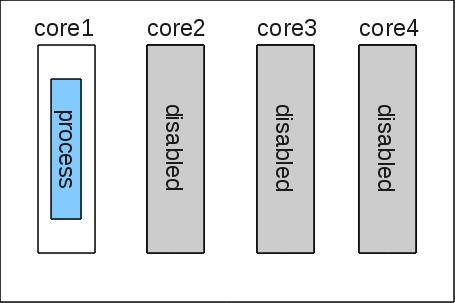
\includegraphics[scale=0.4]{./Figures/disabled_cores.jpg}
    \rule{35em}{0.5pt}
  \caption[Disabled cores]{One core is hosting the MPI process, others are disabled}
  \label{fig:disabled_cores}
\end{figure}
\begin{figure}[htbp]
  \centering
    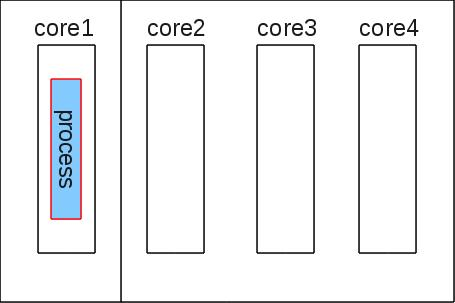
\includegraphics[scale=0.4]{./Figures/bind_to_core.jpg}
    \rule{35em}{0.5pt}
  \caption[Core binding]{None of the cores are disabled, but the
    process is bound to one core, so it doesn't migrate}
  \label{fig:core_binding}
\end{figure}
\subsection{Impact of instrumentation}
In the context of the collection of traces, "instrumenting" an
application means specifying what kind of data we need and which
part of the program we need it from. This can be done either directly
(by inserting function calls or macros that record the data we want),
or by using an overlay library for this purpose. For example, in the
case of TAU, there is a feature called selective instrumentation,
which provides us with the possibility to specify which functions we
want to be traced.\\
When instrumenting the application, it is important to know at what
degree we want to do it. We want to collect the data we need, but the
greater the degree of performance instrumentation in the program, the
higher the likelihood that the performance measurements will alter the
program's performance, an outcome called \emph{performance
 perturbation}.\cite{sm06} In the case of most performance tools, TAU
included, this is a concern that the developers try to address by
reducing the overhead of the performance measurements as much as
possible. It is worth noting though that although the overhead the
measurements cause might be reduced, they can't be completely
eliminated, since the tracing operations have to
be handled by the processor as well. Because of this, the user has to be
very careful when instrumenting an application. There are two main
concerns that come up in our case.
\paragraph{Time overhead}
Instrumentation can have a sizeable negative impact on the performance
of the application. If the instrumentation causes a noticeable
increase in running time, the simulator's prediction might be off,
since it doesn't take into account the instrumentation overhead (as
instrumentation is not part of the experiment).
\paragraph{Impact on hardware counter values}
As mentioned before, when collecting time-independent traces, we use
hardware counters to measure the volume of each operation. The
hardware counter doesn't distinguish between events related to the
experiment and tracing operations, thus all of them are taken into
account. The result is that the collected trace represents the traced
experiment, while we want information from just the experiment,
without the traces. If the difference is too big, this can make our
simulations look inaccurate. The impact it can have when using
off-line simulation, where the simulator replays the traces corrupted
with this overhead is shown in \cite{dms12}.\\[0.5cm]
In \cite{dms12}, the authors propose an instrumentation as a
correction to their previous work in \cite{dmsq11}. The problem was
that there was a sizeable overhead caused mainly by TAU building the
whole call path of the instrumented application. While it can be
very useful when trying to find bottlenecks in the application, this
information is not needed for simulation purposes. In the proposed
method, we tell TAU to exclude all of the source files from the
instrumentation. This way, instrumentation becomes minimal, while
still covering our specific needs: the hardware counter will be
triggered at each MPI call to measure the number of executed
instructions in the operations. All of the information related to MPI
calls, i.e. the id of the process that made the call, the name of the
function and its parameters are traced. All this while both the time
overhead and the hardware counter value discrepancies are considerably
reduced, as shown in \cite{dms12}.
\subsection{Clock synchronization}
\label{sec:clock_synch}
Another obstacle that comes up when wanting to analyze trace data
generated in a distributed system is related to clock
synchronization. When running a parallel experiment on a distributed
system that uses multiple nodes, all the used nodes produce separate
trace streams independently of each other. The problem is that between
the local processor clocks of different nodes, there almost always exists
some amount of discrepancy, mostly related to the temperature
of the processor. No matter how little this discrepancy is,
it can accumulate over time, as well as it can change the logical
event order, which requires a message to be received only after being
sent from the other node. This is also referred to as the \emph{clock
condition}.\cite{wbswpclg00}\cite{brwl09} Such inaccuracy in the traces
can lead to false conclusions when doing the performance
analysis. Even though in our work we want to use time-independent
traces, violations of the clock condition is still a problem we have
to be able to handle.\\
The problem could be easily avoided if every process would use a
global clock instead of the local clock of the node it's running
on. The problem with this approach is that accessing the global clock
can be much more expensive than accessing the local clock, thus
causing performance issues, as well as it's not available on every
platform. In \cite{wbswpclg00}, the authors use an IBM switch
adapter's globally synchronized clock's register to periodically
collect global clock records for each node, thus being able to correct
the local clock discrepancies after the experiment finished.\\
The main problem with this is, as already mentioned, that although
some systems do offer a relatively
accurate global clock, many other systems are only equipped with
processor-local clocks, in which case the problem has to be approached
from another direction. There exist clock synchronization protocols,
such as NTP \cite{m92}, which provides a widely used solution to align
the clocks to a certain degree by adjusting local clocks at regular
intervals to a globally accessible time server. Unfortunately, due to
varying network latencies, this method still leaves an error rate
of about 1 ms when synchronizing, which is not good enough for our
purposes.
TAU handles this problem with another post-processing approach, using
an extended and parallelized version of the \emph{controlled logical
clock} (CLC) algorithm, which is described in \cite{brwl09}. CLC
retroactively corrects clock condition violations in event traces of
message-passing applications by shifting message events in time. When
making such a correction, CLC makes certain precautions, since
after the modification of individual timestamps, the length of
intervals between events in the immediate vicinity of the affected
event might change, as well as new clock violations might be
introduced.\\[0.5cm]
In this chapter, we talked about the reasoning behind why we need a
trace automation framework. We described certain attributes that we
want our tool to have, as well as the current trace collection method
that we'd like to make easier and more straightforward. We also
depicted some of the obstacles that we need to pay attention to when
collecting traces, as well as methods to overcome them. In the next
chapter, we'll discuss more specific details about the implementation
of the framework.
 % Problem Description

\externaldocument{Chapter3}

% Chapter 4

\chapter{Implementation}
\label{Chapter4}
\lhead{Chapter 4. \emph{Implementation}}

In this chapter, we discuss specific details about the implementation
of the framework. First, we talk about testbeds, specifically
Grid'5000, which is the testbed that was used during development. We
discuss the main features of Grid'5000, as well as some important
usage details. The first version of the test framework
is Grid'5000-specific, meaning that it utilizes features that might
be different or might not be present on other platforms. In the long
term, the framework can be developed to eliminate such
dependencies. After that, an example process is described, that
represents a typical use case of our framework: an MPI experiment on
multiple nodes. We also discuss XPflow, the experimentation engine
used for the implementation. We talk about XPflow's approach to
creating workflows, taken from Business Process Management. We
describes how this is applied to our example experiment by depicting
the previously mentioned example process in an XPflow model,
consisting of \emph{processes} and \emph{activities}.
\section{Environment}
\label{sec:environment}
\subsection{The importance of testbeds}
Most Grids that are deployed at a large scale are production platforms
inappropriate for research: such Grids mostly have an environment
that's been
set up specifically for the owner's purposes. Such a system would most
probably need some amount of reconfiguration in order to make it
feasible for what we would like to do, which might influence the
behavior of the system. Another concern is that running experiments on
the platform might cause delays, or even disruption in the
service the Grid is originally used for. Obviously, this is most
probably not acceptable for the owner of the Grid. This is why it is
important to make a distinction between production Grids and Grids
that are made for testing purposes, or "testbeds". Because testbeds
are specifically made for researchers to run experiments on, using up
resources is not that much of a concern as it would be on a production
platform. Since other people might be using the same platform, there
are of course still some limits as to how much resources one user can
utilize, but these limits are not so strict and are much more prone to
negotiation. As previously mentioned, another important factor is that
the nodes we are working on should be reconfigurable: we need to be
able to make customizations to set up our testing environment. We need
to be able to install and uninstall programs. Root access should not
be necessary when doing tests, but it can make things easier,
especially when configuring the environment. Deep control and
monitoring
mechanisms are also needed (not just in one node, but across multiple
nodes) in order to be able to track our experiments.\\[0.3cm]
Simulation with SMPI can be done on any system, since it only needs
one node but in order to run RL experiments, such a testbed is
needed. Most of the work related to this thesis has been done on the
Grid'5000 platform.\cite{bccddjjllmmnpqrtt06}
\subsection{Architecture of Grid'5000}
Below, we discuss some of the architecture aspects of Grid'5000 to
show how it fulfills our previously mentioned needs, as well as how it
addresses some other concerns as well. Description details are taken
from \cite{bccddjjllmmnpqrtt06}.
\subsubsection{Networking}
Grid'5000 is a platform currently consisting of 5000 CPUs, distributed
across 9 different sites in France (figure \ref{fig:g5ksites}),
connected by high speed network. These sites host their own clusters
and they are connected through the internet. It is worth noting that
there are multiple clusters on each site. For example, the
\emph{lille} site hosts the \emph{chimint}, \emph{chirloute} and
\emph{chinqchint} clusters.
\begin{figure}[htbp]
  \centering
    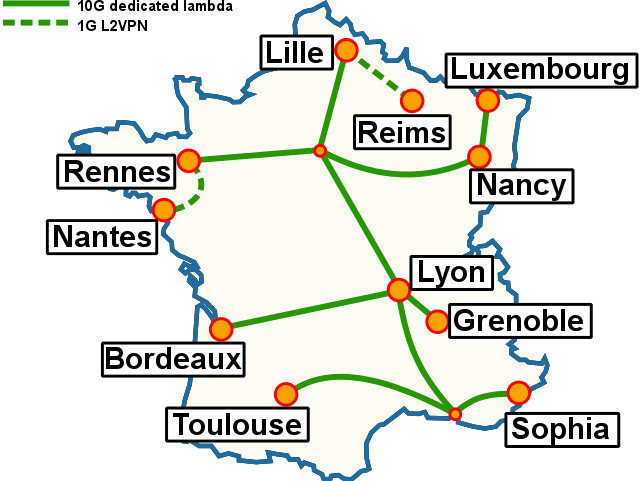
\includegraphics[scale=2]{./Figures/Renater5-g5k.jpg}
    \rule{35em}{0.5pt}
  \caption[Grid'5000 sites]{The sites of Grid'5000}
  \label{fig:g5ksites}
\end{figure}
It is very important with regard to the
experiments that inter-site communication and inter-node communication
are unrestricted and don't weigh any overhead on the
experiments. Thus, all communication can be done without any
constraints between sites. But
as for security, we have to take into account the following: if a
node is fully reconfigurable by the researcher, that means we
can't make any assumptions about the configuration of the security
mechanisms on an allocated node, thus, we have to assume that they are
unprotected. This is the reasoning behind the decision that sites
themselves (thus, of course, the nodes they are hosting) are not
directly connected to the internet, making Grid'5000 an isolated
domain. This way, the sites are protected against DoS attacks.\\[0.3cm]
It is possible to open restricted routes through the internet to
external clusters, which provides the possibility of doing
multiplatform experiments.
\subsubsection{User view and data management}
As previously mentioned, communication is done with minimal
restrictions between Grid'5000 machines, meaning that authentication
procedures in such cases are also minimal: a user has a single account
across the whole platform. An LDAP directory is installed to provide
this in a reliable way. Every site runs an LDAP server. These servers
have the same root and there is a branch for every site. On a given
site, the local administrator has read-write access, as well as is
able to manage user accounts.\\[0.3cm]
A user has access to all of the Grid'5000 sites and services
(monitoring tools, wiki, deployment, etc.). The user also has an
independent home directory at every site. Synchronization of home
directories across different sites can
be done with any of the standard tools, such as \emph{rsync},
\emph{scp}, or \emph{sftp}. Data transfers to the outside world are
restricted - it can only be done via secure tools such as \emph{scp}
in order to prevent identity spoofing. Authentication is done via a
user-generated public ssh key, in order to prevent brute-force
attacks.
\subsubsection{Experiment scheduling}
\label{sec:experiment_scheduling}
At cluster level, the OAR\cite{xdghmmnr05} resource management system is
used to handle the scheduling of experiments and resource
allocation. Large-scale operations such as parallel task launching or
monitoring is handled by a specialized parallel launching tool,
Taktuk\cite{chr09}. Taktuk is a handy tool which can be used from the
console to, for example, perform a certain set of tasks on multiple
nodes, or to broadcast files across them.\\[0.3cm]
A simple grid broker is handling resource management at grid
level, allowing co-allocation of nodes on multiple
clusters. Co-allocation is a very simple process for the user who,
after submitting an experiment needing several sets of nodes across
different clusters, receives an identifier from the broker which can
be used to retrieve all necessary information about the allocated
nodes.\\[0.3cm]
Node reconfiguration, talked about in more detail below, co-operates
with the resource management system at certain points. Such a point is
that when a user submits an experiment that requires node
reconfiguration, the job submission is registered in a queue. Also, in
the prologue script that runs before the actual experiment, deployment
rights are given to the user which gives him/her the capability to
deploy system images on the allocated nodes. An epilogue script runs
after the experiment, revoking these rights. After the experiment is
finished, all of the allocated nodes are rebooted, deploying a default
environment, to provide a constant, unified system to run experiments
on that don't need node reconfiguration.
\subsubsection{Node reconfiguration}
Node reconfiguration on Grid'5000 is handled in a very user-friendly
way, using a tool called Kadeploy3\cite{jsn13}. For every user, a set
of default environments is available at start. After starting an
interactive job (that is, a job that requires node reconfiguration),
the user can deploy any of these environments by providing the chosen
image's name to Kadeploy3. Deployment usually takes only a few minutes
to complete - deployment time obviously increases as we do the
deployment on more nodes. After this, the nodes are rebooted and the
user can log onto any of the nodes where an image was successfully
deployed. When logged in, the user can freely customize the
environment: he/she can
install or remove software, modify configuration files, etc. Root
password is given to all Grid'5000 users as well to provide more
possibilities. After reconfiguring the environment, the user has
the possibility of saving the now customized image. This image
includes all software layers from OS to application levels, just as it
was for the default environments. The home directory is independent of
the image. After successfully saving an image, the user can deploy it
on the allocated nodes the same way he/she did with the default
images. This way, an environment tailored for the specific needs of
the user only needs to be created once, then it can be freely reused
on any other node on the site at a later time. When trying to port an
image created on one site to another site, there can be compatibility
issues due to inter-site differences. Modifications to the customized
image can be done with ease - after modifying the environment, the
user can save it again, with an increased version number. When
deploying the image, the deployment software chooses the highest
version number of the given image by default, but the user is provided
with the possibility of choosing any of the earlier versions.
\section{An example process}
\label{sec:example_process}
A typical example process that we'd like to automate with the
framework is, of course, the acquisition process of real-life (RL)
traces. To reiterate the more detailed description of trace
acquisition (see \ref{sec:rl_traces}), this example process consists
of the
following steps, assuming that we already have a customized image set
up for our tests, as well as we already have an executable benchmark
application we'd like to run:
\begin{itemize}
\item allocate the specified number of nodes on a specified site
\item deploy our custom image on the allocated nodes
\item create a nodefile containing the names of the allocated nodes
\item broadcast the runnable benchmark across the nodes
\item disable all cores but one on every allocated node (see
  \ref{sec:multiple_cores} for explanation)
\item run the mpi experiment from a chosen "head" node (can be any of
  the allocated nodes)
\item gather the traces from the allocated nodes to the head node
\item merge the traces
\item convert merged trace file to Paje format
\end{itemize}
As a side note: in this example, we assume that we are working on the
Grid'5000 testbed. As previously mentioned, most of the work regarding
this thesis was conducted there.\\[0.3cm]
As for the example process: parameters that the user can specify
are the number of nodes, the chosen Grid'5000 site, the image to
deploy, the runnable and the parameters to mpirun (for example to
disable Infiniband) and to the trace\_gather script. The nodefile
created in the 3rd step is necessary for the operations that are
needed to do something on all the allocated nodes.\\[0.3cm]
Now let's take a look at the experimentation engine we'd like to use
for implementing the framework to automate processes like this.
\section{XPflow}
XPflow is an experimentation engine, with one of its main goals being
to provide the possibility to easily automate experiments by creating
workflows. XPflow is a fairly new project. So new in fact, that at the
time of writing this thesis, its source code hasn't been published
yet, although it's going to be released in the very near future.
In 2.8.2, we already discussed business workflows, foreshadowing the
fact that XPflow, the tool used to implement our framework, is based
on that approach, which includes Business Process Modeling and
Management. There are 2 main concepts in XPflow\cite{bn12_2}:
\begin{itemize}
\item Process: It is the high-level description of the experiment,
  written in a DSL, which is embedded in Ruby. Processes are
  responsible for orchestrating activities and other processes,
  creating a workflow.
\item Activities: The low-level building blocks of the
  experiments. They are written in Ruby and used for implementing the
  lower-level details of the experiment, to do the "real work" in it
  (for example: manage files, start the MPI job).
\end{itemize}
Lets take a look at how these concepts are used through
examples, while uncovering a few other possibilities of XPflow.
\subsection{A general example}
First, we examine an example of transforming general, everyday
activities transformed into XPflow (\ref{fig:xpflow_example1}).
\begin{figure}[htbp]
  \centering
    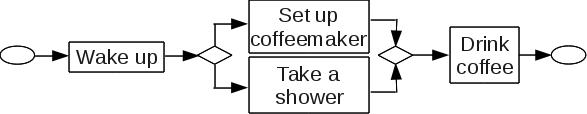
\includegraphics[scale=0.7]{./Figures/xpflow_example1.jpg}
  \caption[Morning routine in XPflow]{Morning routine in XPflow}
  \label{fig:xpflow_example1}
\end{figure}
On the diagram, circles represent the starting and end point of the
process, the rectangles represent activities and the whole diagram
represents a process.\\[0.3cm]
In XPflow, it is possible to execute activities sequentially or in
parallel. An example for sequential execution on
\ref{fig:xpflow_example1} is drinking coffee: the activities preceding
it must all be finished before that activity can be
started. On the contrary, setting up the coffeemaker and taking a
shower can be executed in parallel, since it's not necessary to stand
by the coffeemaker while it finishes - we can take a shower while it's
running.
\subsection{Real-life trace collection example}
After the generic introduction, let's take a look at how we could
represent the experiment we described in section
\ref{sec:example_process} in XPflow. The representation can be seen on
\ref{fig:xpflow_example2}.
\begin{figure}[htbp]
  \centering
    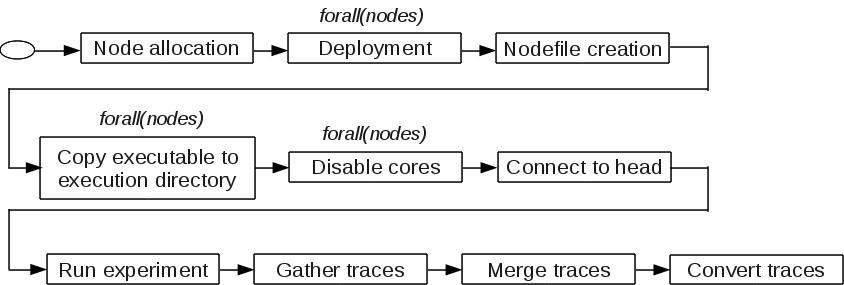
\includegraphics[scale=0.5]{./Figures/xpflow_example2.jpg}
  \caption[MPI experiment example in XPflow]{A typical MPI experiment
    in XPflow}
  \label{fig:xpflow_example2}
\end{figure}
On this representation, there is no parallel execution like in the
previous example: one activity has to be executed sequentially after
the other, the activities depend on each other. However, as we can
see, some of the activities are distinguished by the text
"forall(nodes)" above them. This means that we iterate through all the
allocated nodes, executing the activity on all of them. This is done
in parallel.\\[0.3cm]
As a side note: in the current implementation, this kind of iteration
is realized not
specifically by XPflow, but by the parallel launching tool mentioned
in \ref{sec:experiment_scheduling}, Taktuk\cite{chr09}. This is simply
because it was simpler to implement it that way, because this is a
known and stable solution, while XPflow is under heavy development
currently, thus its internals are subject to change. However, it could
be done with XPflow-specific funcionalities as well. In the long term,
using XPflow-specific funcionality would make the framework more
generic (less Grid'5000-specific).
\section{The framework}
In this section, we talk about the structure of the implemented
framework, its functionalities and usage.
The framework consists of two main parts: there is a frontend and
there is an XPflow structure called a "library" as a backend. While
the expression "library" may sound strange in this context, this is
what comes the closest to a class in XPflow: we are able to store
variables and have member functions, features which the framework
makes much use of.\\[0.3cm]
Below is a more detailed discussion of the most important traits of
the frontend and the backend.
\subsection{Frontend}
The frontend is an interface between the user and the framework. It
has the function calls the user can use when orchestrating an
automated experiment. The example process in \ref{sec:example_process}
contains most of the processes that we'll discuss below.
\subsubsection{init; finish}
These processes need to be called at the
beginning and at the end of the experiment respectively. These methods
have tasks along the lines of variable initialization and metadata
collection. They will be discussed in greater detail when talking
about the backend.
\label{sec:keeping_of_nodes}
\subsubsection{reserve\_and\_deploy}
The allocation and deployment of the nodes are coupled inside one
method. The framework currently is only able to allocate nodes on one
specified site, but the possibility to run experiments on nodes across
multiple
sites could be implemented in the future. It's important to note that
when using XPflow's \emph{reserve\_nodes}, we set the \emph{keep
  => true} argument. This is so we actually keep the job
open until the given time limit expires - we don't kill it at the end
of the experiment. This is so we can use \emph{checkpointing} (see
below) to run other experiments on the same nodes without having to do
the allocation and deployment process again (which can take up several
minutes).
\subsubsection{broadcast}
This method can be used to broadcast any file
across the nodes to a specified destination path. It can be utilized
to broadcast the benchmark runnable to every node to the destination
where the execution will take place. This needs to be done in order
for MPI to utilize all of the nodes - if a runnable is not present in
the place of execution on a given node, MPI won't be able to start its
processes there. For example, if we want to run the experiment and
generate the trace files in the /tmp directory, we will broadcast our
benchmark runnable to /tmp across the nodes.
\subsubsection{disable\_cores}
Disabling cores on nodes can be necessary
as a method to overcome simulation inaccuracy caused by SMPI's
inability to predict the performance of an MPI application when using
multiple cores, as mentioned before, in the \emph{Problem Description}
chapter.\\[0.3cm]
This method, unlike the others in the frontend, is an \emph{activity}
instead of being a \emph{process}. This is done as a workaround to an
XPflow pitfall regarding proxy variables, an issue that will be
discussed in \ref{sec:proxy_variables}.
\subsubsection{mpirun}
This method is for actually running the benchmark
itself. It is important to give the full path to the mpirun runnable
as an argument to the process call, otherwise we can't be sure that
the MPI implementation running is the one we want.
\subsubsection{trace\_gather}
\label{sec:trace_gather}
After running our MPI experiment, the gathered traces are scattered
amongst all the corresponding nodes. This process calls a script
called trace\_gather\cite{ms11} (which needs to be set up on the system
image manually), which copies the traces collected on the
different nodes to the one node we run the script on. We need to call
the script from the path where the execution happened, since that's
where the traces were gathered. After running
this process, we can assume that all the trace files are on the node
we made the function call from. For example if we have our traces in
/tmp, we need to call trace\_gather from there.\\[0.3cm]
Trace\_gather has a parameter called arity. This parameter serves the
purpose of optimization. Trace\_gather
works by logging in to each node in question and then sending its
respective trace file(s) to the requested destination. If the arity is
greater or equal than the number of nodes - 1, then every node sends
its package to the head node - if we imagine sending the traces with
the help of a tree, we could say that the root is the head node, and
all the other nodes are its children. If we specify arity as less than
the number of nodes, we can add extra levels to the tree: some nodes
don't directly send their traces directly to the head node, but to an
intermediate node, which then sends it further up the tree, eventually
getting to the root, the head node.\\[0.3cm]
See figure \ref{fig:tracegather_arity} for an example: in a system
with the total of 8 nodes, we can see on the left how trace\_gather
works if we set the arity to 7 and when we decrease it to 4. In the
first case, all the other 7 nodes send their traces directly to the
root of the tree, the head node (H). In the second case, where the
arity is 4, we split the nodes into 2 groups: the first group of three
have the head node as their parent - they send the traces there
directly. The second group can be seen on the right: 3 of the nodes
form a third level on the tree, with an intermediate parent. These 3
nodes send their traces to that parent node, after which the parent
node sends its traces, coupled with the traces received from its
children, to the root node. With proportionally more nodes, not
sending everything directly to the root can provide a noticeable
performance increase for trace\_gather.

\begin{figure}[htbp]
  \centering
    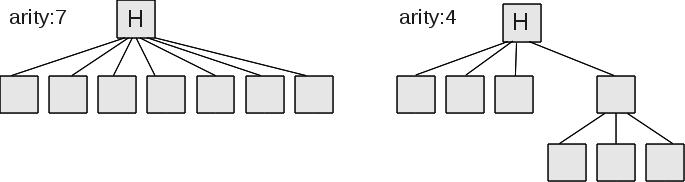
\includegraphics[scale=0.6]{./Figures/tracegather_arity.jpg}
    \rule{35em}{0.5pt}
  \caption[Arity in trace\_gather]{Examples of the trace\_gather's
    algorithm with two different arity values. Every child node is
    sending its traces to its parent.}
  \label{fig:tracegather_arity}
\end{figure}

\subsubsection{execute\_head}
This activity can be used to execute any command on the head node. The
head node is one of the allocated nodes, arbitrarily chosen by the
system. This is the node where the \emph{mpirun} command is run
from.\\[0.3cm]
The \emph{execute\_head} activity is useful for post-processing
purposes, such as calling the TAU\cite{sm06} script
\emph{tau\_treemerge.pl}, which is responsible for merging the traces
into one trace file and the event files into one event file. This is
useful, as after we have one single trace and event file containing
all our traces, we can manipulate them easier.\\[0.3cm]
\emph{execute\_head} can also be used to convert our traces. For
example, Akypuera's\cite{s13} \emph{tau2paje} script can be used to
convert TAU traces to traces visualizable with the Pajé\cite{cob00}
visualization tool.
\subsection{Backend}
As mentioned before, the backend of the framework is an XPflow
construct called a \emph{library}. A library has state, so we can have
internal variables and methods, a functionality that we make use of:
if we couldn't save our state between individual function calls,
certain parameters, such as the number of nodes or the name of the
site we are working on would need to be given every time. Instead, we
can just put those values in variables and use them later when
needed.\\[0.3cm]
Libraries can also contain activities. Most of the "real work" is put
into the library in the form of member activities. The backend
interfaces with the frontend, which makes calls to these activities
whenever needed.
\subsubsection{Metadata}
The backend library is also responsible for handling metadata
collection. Collected metadata includes:
\begin{itemize}
\item the date the experiment was run,
\item the runtime of the experiment,
\item the benchmark that was run,
\item the site and the nodes that were used for the experiment and
\item the image that was deployed on the nodes.
\end{itemize}
Certain elements of this list is provided by the user, while giving
certain parameters to a function call. For example when reserving
nodes, the user has to give the name of the site he/she wants to use,
as well as the name of the image that he/she wants to be
deployed. Other metadata is decided during runtime: a prime example to
this are the nodes used. The user only tells the framework the number
of nodes to allocate - the framework then gives the command on the
system to allocate the nodes, then saves the names of the allocated
nodes in a nodefile, which can be used later as a reference to our
nodes in question. There are also pieces of metadata directly
generated by the framework, such as the date and the runtime of the
experiment. The date is saved in the previously mentioned \emph{init}
method, while the runtime is calculated by saving the starting time in
the \emph{init} method, the ending time in the \emph{finish} method,
then calculating the difference.
\subsection{Checkpointing}
\label{sec:checkpointing}
XPflow has a very useful feature, called checkpointing. A checkpoint
can be put anywhere in our experiment, making it possible that in the
next run, control is \emph{resumed} at the place of the checkpoint. An
example usage can be seen on \ref{fig:checkpoint1}: we put a
checkpoint after the allocation of nodes (line 12). As previously
mentioned in \ref{sec:keeping_of_nodes}, the node allocation is done
in such a way that they remain available even after the experiment is
done. So with putting a checkpoint there, we don't have to wait
through the several minute long node acquisition and deployment
process each time we want to run an MPI experiment: we can re-run it
on the same allocated nodes, as long as the time limit we set at the
node allocation allows us. It is also possible to change the code
after the checkpoint to run some other experiment, as it can be seen
on \ref{fig:checkpoint2}: there, we modify the code so it runs
\emph{dt.A.2} instead of \emph{lu.A.2}. We had to modify the code in
two places to achieve this: first, we need to broadcast the other
benchmark across the nodes (line 14) and the path to the runnable
needs to be changed as well when giving the command to run the
experiment (line 19). If the time interval we allocated the nodes for
passes, we have to run that part of the experiment again. This can be
done by telling XPflow to ignore the checkpoints (with the argument
\emph{-I}). In our example, this time interval is 30 minutes, as it
can be seen on line 10, where we give it as a parameter to the node
acquisition process.
\begin{figure}[htbp]
  \centering
    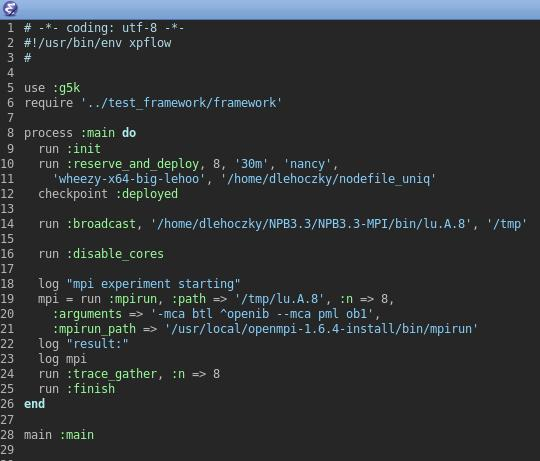
\includegraphics[scale=0.7]{./Figures/checkpoint1.jpg}
    \rule{35em}{0.5pt}
  \caption[Checkpoint example]{Example usage of checkpointing}
  \label{fig:checkpoint1}
\end{figure}
\begin{figure}[htbp]
  \centering
    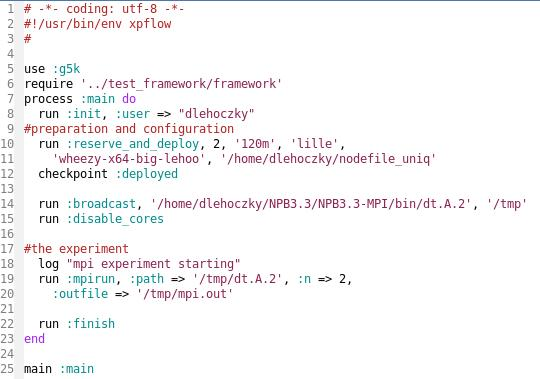
\includegraphics[scale=0.7]{./Figures/checkpoint2.jpg}
    \rule{35em}{0.5pt}
  \caption[Checkpoint example - code modification after checkpoint]{We
    can modify the code that comes after the checkpoint}
  \label{fig:checkpoint2}
\end{figure}
\subsection{Proxy variables}
\label{sec:proxy_variables}
There is a shortcoming of XPflow that caused a little headache during
the development of the framework. The problem stems from
the fact that the XPflow processes are written in a DSL that is
embedded in Ruby. Ruby is very
flexible in that regard, but one unsolved problem is that the body of
the process blocks are executed \emph{before} the execution of the
process itself. The problem with this is that at the time of the
execution of the process blocks, some of the variables that the
process uses contain only some proxy value, not the value that
was actually put in there. This problem has been briefly mentioned when
talking about the \emph{disable\_cores} method. In that particular
method, multiple command strings are needed, containing the commands
that are needed to be executed to disable the cores on the nodes. In
these command strings, the variable containing the nodefile is needed
to be inserted. If \emph{disable\_cores} was a process, this variable
would contain only a proxy variable at the
time we want to insert it in the string, even if we would put the
correct value in it right before. Writing this method as an activity
instead of a process solves this problem, since activities are written
in plain Ruby.\\[0.5cm]
This chapter was about the implementation details of the
framework. First, we talked about the development and testing
environment, the Grid'5000 testbed. We went over its architecture and
its features deemed to be the most important for this project. After
that, we constructed an example process for real-life trace
collection, which was used when portraying the features of the
experimentation engine, which the framework was developed with:
XPflow. We talked about why XPflow is feasible for our project and its
main features, through two examples: one basic, general example and
one that is very relevant to our case, the aforementioned RL trace
collection example. After that part, we talked about the architecture
of the implemented framework, and some of its methods. In the end, we
mentioned metadata collection as an important feature of the
framework, as well as checkpointing, an XPflow feature that proved to
be really useful during development.
 % Implementation

\externaldocument{Chapter4}
\externaldocument{Chapter3}

% Chapter 5

\chapter{Evaluation}
\label{Chapter5}
\lhead{Chapter 5. \emph{Evaluation}}

\label{sec:evaluation_plan}
In the first part of this chapter, declare the most important
specifics about the process of the evaluation of the
implemented framework, the goal of which is to make
conclusions about whether or not we succeeded in achieving the
requirements we specified earlier. The evaluation will be done by
running a multi-step, fairly typical experiment both manually and with
the framework, so we can easily observe the differences.\\
After specifying the process, we will go over the results of the
evaluation. First comes the part where we discuss the
results we got when running the experiment using the framework. Here,
we describe how the experiment was orchestrated: what processes were
used, how the test file's code looked like. Then we'll take a look at
how the experiment was run, what information was given to the user
during runtime and how much time it took. Then, we will go over the
steps of the experiment done by hand, starting from connecting to the
interactive job started by the framework previously, then proceeding
with the experiment, including a summary about what commands
were needed to be given and how much time the steps took. After that,
we'll compare the results concerning runtime and the produced traces,
including making observations about the visualizations. Then we
compare the two different methodologies used: the "old", manual method
with the usage of the newly implemented framework. By comparing the
methodologies, we try to draw a conclusion whether or not the usage of
the framework is more feasible in the long term than the manual
method. In the end, we take a look at the most important shortcomings
of the current version of the implementation, as well as ideas about
how we could overcome them.
\section{Methodology}
The experiment process used in the evaluation will consist of the same
steps as mentioned before in the Implementation chapter as an example
MPI experiment process (see \ref{fig:xpflow_example2}), used to collect
RL traces, which can be used for example for the development of
SMPI. The steps in the process are very generic though: we need to be
more precise about certain details of the experiment.
\subsection{Experiment specification}
\subsubsection{Prerequisites}
There are certain prerequisites that are assumed about the user's
environment when running the experiment.
\begin{itemize}
\item XPflow is needed to be present at the place of the execution of
the test. This can be the user's workstation or any feasible
environment.
\item In order to provide authentication without prompting for a
password, ssh-keys are needed to be configured correctly
  \begin{itemize}
  \item between the place of execution and the site,
  \item between the site and the nodes,
  \item and between the nodes (required by mpirun and trace\_gather).
  \end{itemize}
\item An image providing the feature described in \ref{sec:image}.
\item The benchmark to run is needed to be compiled and available in
  the path that we give the broadcast method of the benchmark.
\end{itemize}
If all these requirements are fulfilled, the experiment should run
without a problem.
\subsubsection{The benchmark}
The benchmark used for evaluation is taken from the NAS Parallel
Benchmarks suite\cite{jfy99}, which is a small set of benchmarks
designed for performance testing of parallel systems. The benchmark
chosen for our current purpose is called \emph{lu.B.8}. The name
consists of 3 parts. The first part, \emph{lu} indicates what the
experiment is about: as its name suggests, the LU benchmark solves a
system of equations represented with a matrix, with the LU
factorization method.\\
The second part of the name, \emph{B} is an
indication about the complexity of the problem that the benchmark
solves. The NPB suite defines so-called "problem classes" for its
benchmarks. B is in the middle "standard" complexity category, being
more complex than the Small (S), the Workstation-size (W) and A, the
least complex "standard" problem size, but less complex than C and the
larger test problem sizes.\cite{d13}\\
Finally, the number \emph{8} at the end of the benchmark's name
indicates how many parallel processes it is intended for to be solved:
for our purposes, we choose it to be 8, thus, we will allocate 8 nodes
for our experiment, each of them running 1 MPI process to solve the
problem.\\
It's important to note that when doing the experiment, we assume that
the benchmark is already compiled, in a specified place in the user's
home folder, provided as a parameter to the broadcast method:
/home/dlehoczky/NPB3.3/NPB3.3-MPI/bin/lu.B.8. As a side note: for the
user \emph{dlehoczky}, the environment variable \emph{\$NPB\_DIR} is
set to /home/dlehoczky/NPB3.3/NPB3.3-MPI, thus it can be used as a
shortcut when accessing the benchmark.
\subsubsection{The environment}
For our experiment, we use the Grid'5000 testbed, discussed in greater
detail before, in \ref{sec:environment}. As we said before, there are
many different sites to choose from. During development,
many tests were needed to be done. Sometimes one or two sites were
undergoing maintenance or became unstable for various reasons. Towards
the end of the development process, the Lille site proved to be
reliable in terms of availability, this is why it was chosen as the
site to run our final tests on.
\subsubsection{The OS image}
\label{sec:image}
We use a customized image called
\emph{wheezy-x64-big-lehoo}. This image contains all the necessary
tools required to run the described process. These tools were
mentioned before, at \ref{sec:rl_traces}, when we talked about how to
collect RL traces, which this experiment is about. To reiterate, let's
sum up what our customized image contains in order to execute our
experiment process:
\begin{itemize}
\item OpenMPI 1.6.4;
\item the \emph{TAU}\cite{sm06} profiling tool;
\item the PAPI\cite{mbdh99}\cite{lmmsl01} interface to low-level
hardware counters (configured so it's linked to TAU, which uses it for
tracing);
\item the \emph{Program Database Toolkit (PDT)}\cite{lcmsmrr00} (also
configured to be linked to TAU);
\item the \emph{trace\_gather}\cite{ms11} MPI program;
\item \emph{Akypuera}\cite{s13}, a library to trace mpi applications
and generate paje trace files. (In our experiment, we only use
its \emph{tau2paje} trace converting script.)
\end{itemize}
\subsubsection{The experiment process}
\label{sec:experiment_process}
As mentioned before, the experiment process will consist of the same
steps as in the example discussed before
(see \ref{fig:xpflow_example2}).\\
To prepare our experiment process, we start by
logging in to the frontend with our user. Then, we start an
interactive job, allocating the desired number (in our case, 8) of
nodes for a specified amount of time. We won't specify what nodes we
want, the system will decide which ones we get. Since there might be
performance disparities between two different sets of nodes, we make
sure to use the exact same set of nodes in the two experiments (the
one done manually and the one done with the framework). We do this by
running the experiment with the framework first, then connecting to
the job started by the framework and repeating the experiment
manually, starting from the deployment part. The node allocation is
not really an important part of the experiment, thus, it's not a
problem that it's omitted from the manual execution.\\
As part of the process that we conduct in both experiments, first, we
deploy the previously mentioned (\ref{sec:image}) customized image on the
nodes. Then we broadcast the runnable (\emph{lu.A.8}) to every node's
/tmp directory. After that comes the step where we disable all but one
core on every node. The reasoning for this step has been discussed
previously (see \ref{sec:multiple_cores}). This concludes the
preparation stage.\\
It is worth noting that, just like we did before at the
checkpointing example (see \ref{sec:checkpointing}), we put a
checkpoint right after deployment. This way, if we want to do another
experiment, we can reuse our already allocated and deployed
nodes. Since deployment is the longest process in the experiment, such
a checkpoint can come in really handy. As already discussed before, we
can modify anything in the experiment that comes after the checkpoint
- the execution will resume and execute the modified code.\\
After the preparation stage comes the execution of the benchmark. We
use OpenMPI 1.6.4, installed on our image.\\
After the running of the benchmark, comes the post-processing. If we
compiled our benchmark correctly with TAU, one trace file (.trc)
and one event file (.edf) is generated for each MPI process. The
traces are generated on the node of execution. This is why first,
we run the \emph{trace\_gather}\cite{ms11} script to collect the traces
and event files scattered across all the allocated nodes to the head
node. When we have all the files on our head node, we use
TAU's \emph{tau\_treemerge.pl}, which is a script that merges all our
trace files and event files into one trace and event file
respectively, also trying to account for any clock skew
(see \ref{sec:clock_synch}) between the trace files with
post-processing methods. Finally, when we have one merged trace and
one event file, we can convert our TAU trace to a format that is
compatible with the Pajé\cite{cob00} visualization tool. Visualizing
the traces makes it easier to analyze and compare. For the conversion,
we use Akypuera's\cite{s13} \emph{tau2paje} script.\\[0.5cm]

\section{Results}
In this part of the chapter, we go over how the experiments went by
observing their different stages. Then compare the results, the
two different methodologies and we discuss the shortcomings of the
framework.
\subsection{Experiment using the framework}
First, we discuss the experiment orchestrated with the test
framework. The test written with the framework consists of one single
file, containing 1 method (the main) and 11 function calls. We can
look at the code on figure \ref{fig:experiment_code}.\\
The experiment itself can be divided into three main stages: the
preparation/configuration stage, the benchmark stage and the
post-processing stage.

\begin{figure}[htbp]
  \centering
    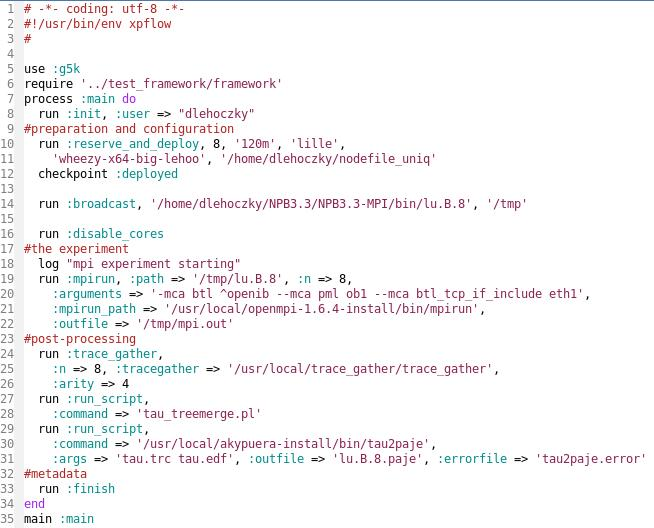
\includegraphics[scale=0.7]{./Figures/experiment_code.jpg}
    \rule{35em}{0.5pt}
  \caption[Experiment code]{The experiment, orchestrated with the test
    framework.}
  \label{fig:experiment_code}
\end{figure}

\subsubsection{Preparation}
\paragraph{Experiment initialization}
In the beginning of every experiment, the \emph{init} method has to be
called in order to configure certain variables with default values and
also to make configuration steps regarding metadata collection
(e.g. record the date of the experiment, the exact time of starting,
etc.). Also, here is where the user can set his/her username to log in
to the nodes. If not set, the username will default to root.
\paragraph{Reserve and deploy}
This is the part where the program starts a job by allocating 8 nodes
on the \emph{lille} site and deploying the image (given as a parameter
to the method) on them. We set the allocation time to 120 minutes (2
hours), which should give us plenty of time to execute the experiment
with both the framework and manually on the nodes.\\
As part of the process, a so-called 'nodefile' is created, which
contains the names of all the nodes that we allocated. Originally, the
environment variable \emph{\$OAR\_FILE\_NODES} is set on the frontend
when logged in to an active job, with the value of the path to a file
containing the node names, each as many times as many cores they
have. During the experiment, we create a nodefile that only contains
each node once, so it can be used as a machinefile for certain
commands later. We specify a custom path to the nodefile with an
argument. If that argument is not set, our nodefile would be created
in the home folder anyway.\\
Logs of the deployment process can be seen on
figure \ref{fig:fex_deployment}. As we can see, we allocate 8 nodes
for 2 hours of time. This means that after 2 hours, the job terminates
and we are disconnected from the nodes. In our case, the 2 hours
proved to be more than enough to conclude our tests. We can also
observe that while the node allocation only took a mere 22 seconds,
image deployment was taking much longer: it went on for about 8
minutes. In the end, we can see the "deployment complete" message,
notifying us that the image deployment process was successful and we
can now move on to the next stages of the experiment.

\begin{figure}[htbp]
  \centering
    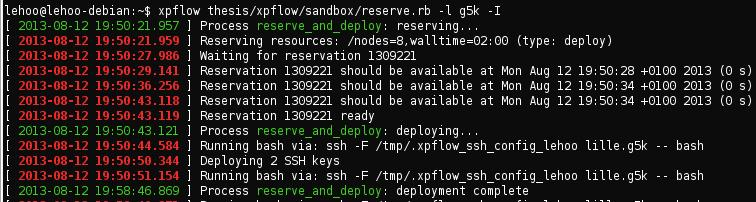
\includegraphics[scale=0.6]{./Figures/fex_deployment.jpg}
    \rule{35em}{0.5pt}
  \caption[Allocation and deployment]{Logs of the node allocation and
    image deployment process.}
  \label{fig:fex_deployment}
\end{figure}

\paragraph{Broadcasting the runnable}
The benchmark needs to be copied to every node to the path where the
execution will take place - otherwise MPI wouldn't be able to start
its processes on every node. The parameters here are pretty
straightforward - we give the method the path to the compiled
benchmark and the path to copy it to. The nodefile is not needed to be
given, since it's already been created and stored by the library
before.\\
As it's a relatively fast and simple process, the framework doesn't
display any extra log messages to notify us of their success. Since
the benchmark was able to run, we can be sure that it succeded.
\paragraph{Disabling cores}
This is the method call that is responsible for disabling all but one
core on every node that takes part in the execution. We talked about
why this is necessary earlier, see \ref{sec:multiple_cores}. No
parameters are needed to be given here.\\
This, like the broadcasting process, is a fast and relatively simple
process. Also, as previously mentioned, the fact whether or not the
cores were successfully disabled is checked in a loop, repeating the
disabling step until it's successful. Thus, we can be sure that this
step succeeded.
\subsubsection{Running the benchmark}
After all the configuration steps have been successfully done, it's
time for actually running the benchmark. As parameters, we first give
the \emph{mpirun} method call the path to the runnable (meaning, of
course, the path that we broadcasted the runnable to before, not its
original path) and the number of nodes, which, in our case, is 8. We
also specify the MPI runnable with its full path: this is to avoid
confusion about which version of MPI is actually running on the nodes,
ensuring that it's the version we deployed on the image (OpenMPI
1.6.4). If not given, it would be defaulted to simply 'mpirun'. We
specify the file to put the output of the benchmark to as well.\\
We can put any extra arguments that we want to give to mpirun in the
"arguments" parameter. In this case, we use this parameter to specify
that our benchmark must not use Infiniband. This is needed because
SMPI is unable to simulate Infiniband connection, thus, a trace
acquired using it would show significantly better performance than the
simulated version.\\
We can see logs produced when running the MPI benchmark, on
figure \ref{fig:fex_mpirun}. At the beginning of the method, the
framework logs the name of the designated head node, which is the node
the benchmark execution commands will be given and where the traces
will be gathered, merged and converted. This node, in our case, is the
node called \emph{chimint-6}.\\
The execution time of the benchmark was 46.769 seconds. This result is
taken from the traces themselves, as we can see see below, at the
visualization of the traces.

\begin{figure}[htbp]
  \centering
    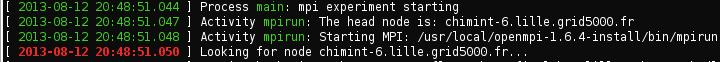
\includegraphics[scale=0.6]{./Figures/fex_mpirun.jpg}
    \rule{35em}{0.5pt}
  \caption[Benchmark execution]{Logs about the execution of the
    benchmark.}
  \label{fig:fex_mpirun}
\end{figure}

\subsubsection{Post-processing}
\paragraph{Gathering the traces}
As we mentioned before, in \ref{sec:experiment_process}, since we
compiled our benchmark with TAU, every MPI process produces
one trace (.trc) and one event (.evt) file. These traces are scattered
across the nodes. To gather them to one node, we use
the \emph{trace\_gather} MPI program. The method call with the same
name takes as parameter the number of nodes, the path to
the trace\_gather executable (the MPI executable is remembered
from the \emph{mpirun} call) and the arity parameter
(see \ref{sec:trace_gather}).
\paragraph{Merging the traces}
For running \emph{tau\_treemerge.pl}, we use the \emph{run\_script}
method of the framework, which is a generic method that executes the
command given as parameter on the head node. No other arguments are
needed in this case. Although we could specify files to put the output
and the error messages to, we don't really need that in this simple
case. The directory to merge the traces in defaults to "/tmp", so that
is not needed either. As we mentioned before, this script doesn't only
merge our traces, it also attempts at accounting for any clock skew.
\paragraph{Converting the traces}
As mentioned before, we use Akypuera's\cite{s13} \emph{tau2paje}
script to convert our traces to Pajé-visualizable format. For this, we
use the \emph{run\_script} method again, giving it the trace and event
files as arguments, as well as files to put the output and the error
messages to. Tau2paje generates error messages because of
synchronization problems (clock skew). As we described before
(see \ref{sec:clock_synch}), clock skew problems are really hard to
overcome. Although the merging script before tried to take care of the
problem, it can't eliminate it completely, but it does a well enough
job so this problem doesn't interfere with the conversion results in
any noticeable way.\\
After the conversion is done, the visualizable trace file called
\emph{lu.B.8.paje} is available on the /tmp folder of the head
node. We can now copy it to our local machine and visualize the
result. (The results will be discussed below, after discussing the
manual experiment.)\\
We can see logs about the post-processing part on
figure \ref{fig:fex_postprocessing}. We can see by the lines starting
with "Looking for the node chimint-6...", that the head node is the
same throughout the experiment, and the post-processing indeed happens
there. We can also observe that the post-processing takes about 30
seconds to complete.

\begin{figure}[htbp]
  \centering
    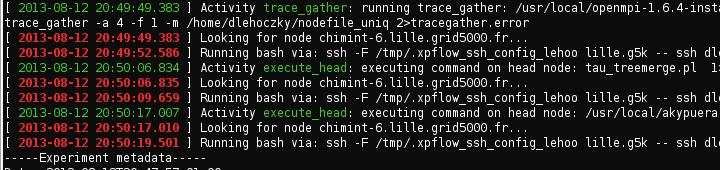
\includegraphics[scale=0.6]{./Figures/fex_postprocessing.jpg}
    \rule{35em}{0.5pt}
  \caption[Post-processing]{Logs about the post-processing part of the
    experiment.}
  \label{fig:fex_postprocessing}
\end{figure}

\subsubsection{Metadata}
In the end, we get some amount of metadata generated by the
experiment, summarizing some of its most important specifics, as it
can be seen on figure \ref{fig:fex_metadata}.\\
It's worth pointing out that the framework keeps track of the time
before and after the checkpoint, which was placed at the
deployment. This way, we can easily distinguish between the time the
deployment took and the time the other parts of the experiment
took. It is obvious by looking at the times that the deployment
process is the longest part of the experiment.\\
If we take a look at the nodes used, we can see that we used nodes
from 2 different clusters on the lille site: the
clusters \emph{chirloute} and \emph{chimint}.

\begin{figure}[htbp]
  \centering
    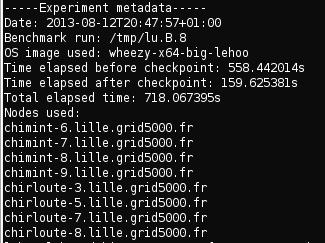
\includegraphics[scale=0.7]{./Figures/fex_metadata.jpg}
    \rule{35em}{0.5pt}
  \caption[Metadata]{Metadata produced by the framework about the
    experiment.}
  \label{fig:fex_metadata}
\end{figure}

\subsection{Experiment by hand}
Now, let's take a look at how the manual experiment went. As mentioned
before, the two experiments consist of the same exact steps. As
before, we divide the experiment into three main sections:
preparation stage, benchmark stage and post-processing stage.
\subsubsection{Preparation}
Below is a table summarizing the results for the preparation and
configuration stage. The whole preparation stage took place on the
frontend of the site "lille", with the user "dlehoczky".
\renewcommand{\arraystretch}{1.5}
\begin{center}
\begin{spacing}{1}
\begin{tabular}{| p{4cm} | p{8cm} | l |} \toprule
  \multicolumn{3}{ |c| }{\textbf{Preparation}} \\ \midrule
  \multicolumn{1}{ |c| }{\emph{Task}} & \multicolumn{1}{ |c|
  }{\emph{Command}} & \multicolumn{1}{ |c| }{\emph{Time
  (s)}}\\ \midrule
  Reserving nodes & Omitted - joined the existing job,
  using the already allocated nodes & - \\
  Deployment & \texttt{\small kadeploy3 -f \$OAR\_FILE\_NODES -e
  wheezy-x64-big-lehoo} & 453.343 \\
  Create a nodefile containing all the node names only once
  & \texttt{\small cat   \$OAR\_FILE\_NODES | uniq > \textasciitilde
  /nodefile\_uniq} & 0.004 \\
  Broadcast of runnable & \texttt{\small taktuk -l dlehoczky -f
  \textasciitilde /nodefile\_uniq broadcast put
  { \$NPB\_DIR/bin/lu.B.8 } { /tmp }} & 0.389 \\
  Disabling cores & \texttt{\small taktuk -l root -f /home/dlehoczky/nodefile\_uniq
  broadcast exec [ 'for i in /sys/devices/system/cpu/ cpu[1-9]*/online;
    do echo 0 > "\${i}" ; done' ]} & 1.974 \\
  \emph{Optional}: Check if the cores have been disabled accordingly
  & \texttt{\small taktuk -f \textasciitilde /nodefile\_uniq broadcast
  exec [ 'cat /proc/cpuinfo' ] | grep process | awk '{if(\$9>0)
  print \$1}' | uniq | awk -F".fr-" '{print \$1".fr"}'} &
  1.319 \\ \midrule
\end{tabular}
\end{spacing}
\end{center}

As a side note: when doing the core disabling with the framework, the
program repeats the disabling step until it confirms it to be
successful, with the step marked as "Optional" here. In the step where
we check if the cores are disabled, every node name is displayed that
has more than 1 core running. The disabling step needs to be repeated
until we don't see any node names when running that command. When
running the test, the disabling step was successful the first time,
thus there was no need to repeat that step.
\subsubsection{Running the benchmark}
Below is the table about the command that was given to run the
benchmark (which is exactly the same as it was for the framework), as
well as its runtime. The benchmark had to be run from the directory
the benchmark was broadcasted to (/tmp in our case), on the designated
head node (which was, in our case, \#{TODO: head node}, the same as it
was for the framework.

\begin{center}
\begin{spacing}{1}
\begin{tabular}{| p{4cm} | p{8cm} | l |} \toprule
  \multicolumn{3}{ |c| }{\textbf{Running the benchmark}} \\ \midrule
  \multicolumn{1}{ |c| }{\emph{Task}} & \multicolumn{1}{ |c|
  }{\emph{Command}} &   \multicolumn{1}{ |c| }{\emph{Time
  (s)}}\\ \midrule
  Running the benchmark
  & \texttt{\small{/usr/local/openmpi-1.6.4-install
  /bin/mpirun -mca
  btl \textasciicircum openib --mca pml ob1 -machinefile
  \textasciitilde /nodefile\_uniq -np 8 /tmp/lu.B.8 1>/tmp/mpi.out}}
  & 46.559 \\ \midrule
\end{tabular}
\end{spacing}
\end{center}

\subsubsection{Post-processing}
After executing the benchmark, the produced traces are sitting on
their respective nodes. Below, we summarize how the post-processing of
the files went. This stage of the experiment, as it was for the
benchmark, was executed on the head node, from the /tmp directory.

\begin{center}
\begin{spacing}{1}
\begin{tabular}{| p{4cm} | p{8cm} | l |} \toprule
  \multicolumn{3}{ |c| }{\textbf{Post-processing}} \\ \midrule
  \multicolumn{1}{ |c| }{\emph{Task}} & \multicolumn{1}{ |c|
  }{\emph{Command}} & \multicolumn{1}{ |c| }{\emph{Time
  (s)}}\\ \midrule
  Gathering the traces & \texttt{\small/usr/local/bin/mpirun
  -machinefile \textasciitilde /nodefile\_uniq -np 8
  /usr/local/trace\_gather/trace\_gather -f 1 -a 4 -m \textasciitilde
  /nodefile\_uniq} & 8.152 \\
  Merging the traces & \texttt{\small tau\_treemerge.pl} & 3.967 \\
  Converting the trace to Pajé-compatible format & \texttt{\small
  /usr/local/akypuera-install/bin/tau2paje tau.trc tau.edf
  1>lu.B.8.paje 2>tau2paje.error} & 10.532 \\ \midrule
\end{tabular}
\end{spacing}
\end{center}

As mentioned previously at the end of the experiment with the
framework: after the conversion process, the file \emph{lu.B.8.paje}
is available on the head node, in its /tmp folder. Now, we can use
scp, rcp or some other program to download it to our local machine
from the remote node.
\section{Comparison}
\subsection{Comparison of results}
First, let's take a look at how much time the experiments took. Below
is a table summarizing the elapsed time for both experiments.

\definecolor{light-gray}{gray}{0.90}
\begin{center}
\begin{spacing}{1}
\begin{tabular}{| c | c | c |} \toprule
  \multicolumn{1}{ |c|
  }{\multirow{2}{*}{\Large \textbf{\emph{Stage}}}} & \multicolumn{2}{
  |c| }{\textbf{\emph{Time (s)}}} \\ \cmidrule{2-3}
  & \multicolumn{1}{ |c| }{\emph{Experiment
  with the framework}} & \multicolumn{1}{ |c| }{\emph{Manual
  experiment}}\\ \midrule
  Preparation & 558.442 & 457.03 \\
  Running the benchmark & 46.767 & 46.559 \\
  Post-processing & 30.118 & 22.651 \\ \midrule
  The whole experiment & 635.327 & 526.24 \\ \midrule
\end{tabular}
\end{spacing}
\end{center}

We can see that although the preparation steps and the post-processing
took more time with the framework, the actual running of the benchmark
took the same amount of time. The time difference in the preparation
is most likely caused by disparity availability of resources to do the
deployment, and the fact that in the second case, we didn't have to do
the node allocation. Another likely reason, that applies to the
post-processing part as well, is simply the fact that we're doing
real-life traces and as such, running time can be different, as well
as results can differ. This is especially true for distributed
systems, where the exact sequence of messages sent is never the same,
in our case, between 8 nodes.
Now, let's take a look at the generated traces. We can see the traces
for both experiments, visualized with Vite, a Pajé visualization tool
on figures \ref{fig:fex_traces} and \ref{fig:mex_traces}.

\begin{figure}[htbp]
  \centering
    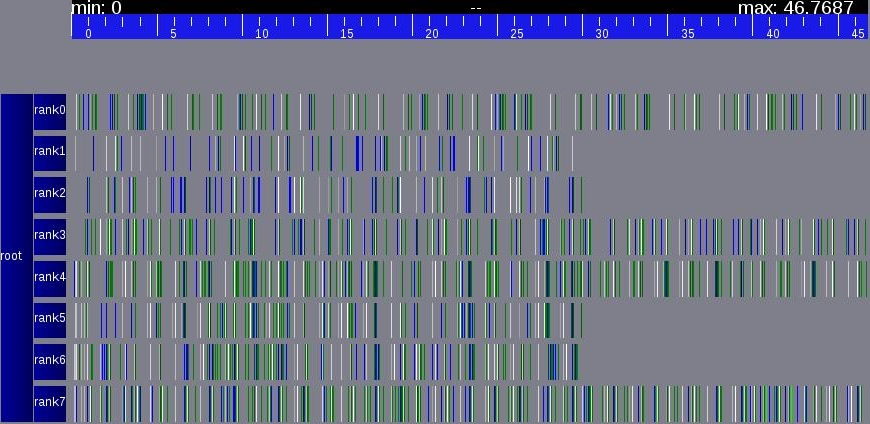
\includegraphics[scale=0.7]{./Figures/lu_B_8_framework.jpg}
    \rule{35em}{0.5pt}
  \caption[Traces from the experiment run with the framework]{Traces
    from the run with the framework, visualized with Vite.}
  \label{fig:fex_traces}
\end{figure}

\begin{figure}[htbp]
  \centering
    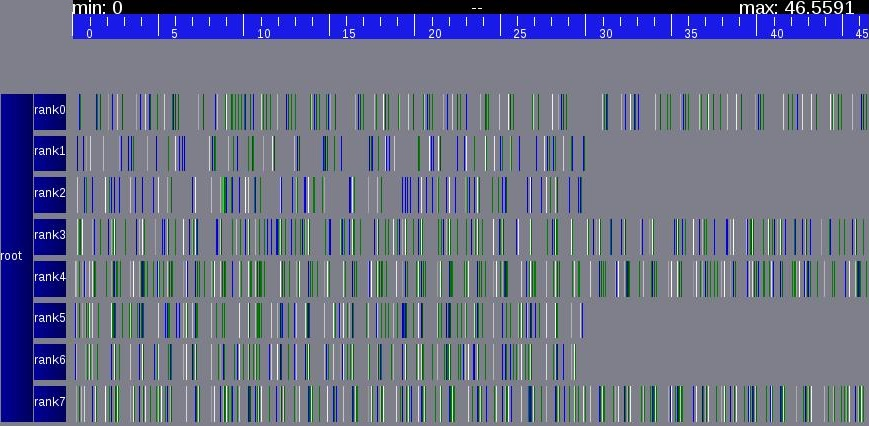
\includegraphics[scale=0.7]{./Figures/lu_B_8_manual1.jpg}
    \rule{35em}{0.5pt}
  \caption[Traces from the experiment run manually]{Traces from the
    run manually, visualized with Vite.}
  \label{fig:mex_traces}
\end{figure}

At first glance, it is apparent that the visualizations are made up of
differently colored lines. These lines represent the different MPI
operations. The X axis is the time. We can see that it starts from
zero, and ends at the time period equal to the benchmark's
runtime. The Y axis represents the different MPI processes, identified
by their rank - we can see the different ranks on the left side. Each
rank forms a horizontal "stripe" of its own, with the MPI operations
belonging to it inside that stripe. As for the MPI operations
themselves: the send operations (MPI\_Send()) are blue, the receive
operations (MPI\_recv()) are green, and the wait operations
(MPI\_Wait()) are white in color.\\
If we observe the two trace visualizations, it is apparent that there
are obvious differences between them - the MPI operations didn't
happen at the same time. Sometimes, one of the experiments executed
more operations than the other in the same time interval and vice
versa. But if we disregard the smaller details, it's also visible that
the two visualizations are indeed very similar to each other: in both
cases, after roughly 29 seconds of execution time, only the processes
with the ranks 0, 3, 4 and 7 continue to execute operations. Due to
the nature of the benchmark, only 4 processes are used from that time.
\subsection{Comparison of methodology}
In the section before, we made the observation that the two methods -
the manual and the one with the framework - produce similar
results. Now the question remains: how do the two methods fare against
each other in other terms, not directly tied to the correctness of the
test results, but rather tied to the methodology.
\paragraph{Reliability}
The problem with the manual method in this regard is that it's
repetitive work and all the commands have to be given individually,
with certain modifications here and there. An obvious advantage for
the framework in this regard is that if it was working once, it will
be working again if we don't modify anything. If something is wrong,
but wasn't wrong the last time, we can be sure that the environment is
at fault - with the manual method, we can never be sure in that, as
there is always the chance that we mistyped something or left a step
out of the process this time.
\paragraph{Reusability}
This is strongly tied to the previous paragraph: after we write a
test's code with the framework, we can save that code and execute it
as many times as we want. We can't do that with the manual steps,
where we have to give the same commands individually again and
again. Bash history and scripts can help our work, but the more
experiments we do, the harder it's going to be to organize
them. Experiments written using the framework can be also organized
into higher-level workflows, providing the potential to run as many
tests as we need, one after the other. The only thing we need to pay
attention to is to correctly store our traces: making sure to copy
them to a more permanent location, each given a unique name, as well
as providing enough space to store all of them - trace files get
proportionally larger, the more complex and more large scale our
problems are.
\paragraph{User interaction}
Although this might seem to be a minor concern, in the long run, this
advantage of the framework can prove to be most valuable: when running
experiments manually, the user needs to pay attention to when the
command he/she gave finishes executing, then input the other command,
right until the end of the experiment. While when using the framework,
we only need to start the execution, which will then, as we saw,
automatically executes the consecutive steps, freeing up the user to
do other things while it's running. We can even set up our experiment
so it copies the traces to its permanent location, so we needn't to
worry about that either. As mentioned before, we can also tie together
multiple experiments into a single workflow easily. And this is
exactly what our main goal was at the beginning: to make the
researchers' lives easier.
\paragraph{Testing speed}
Again, this is closely tied to other viewpoints already mentioned. Due
to the fact that no user interaction is required, as well as the fact
that we have the possibility to run as many benchmarks in a single
workflow as we want, we can potentially run proportionally more
benchmarks, thus producing proportionally more traces and results in
other forms, which, as mentioned before, is much needed in our case
for validating SMPI.\\[0.5cm]
In this chapter, we first went over the specifics of the evaluation of
our implementation. We talked about the chosen benchmark to
gather traces from. We also discussed what the chosen
environment is going to be (Grid'5000) and what operating system image
we are going to deploy on our nodes before running the benchmarks on
them. After that, we went over the experiment process: the RL trace
collection for a given benchmark. We mentioned that our experiment
process will be done using two methods: we run it with and without the
framework to demonstrate how the two methods differ from each
other, in order to make a conclusion about whether or not it's worth
to use our implementation. Then we went on to discuss the process
itself: the preparation steps, the running of the benchmark and the
post-processing part.\\
The section after that was about the results of running the
experiment with the two methods. We first went over the experiment
orchestrated with the framework in detail: we observed how the code
looked like, then went on to discuss the different stages: the
preparation and configuration stage, the running of the benchmark and
the post-processing stage, then taking a look at the metadata
produced. After that came the manual experiment. Similarly, we went
through the stages, this time summarizing what the commands and the
elapsed time were for each step. Then we went on to compare the two
methods: first, we compared the results, taking into account both the
elapsed time and the collected traces. We made observations about the
visualizations, concluding that the results were very similar,
although there are differences in details such as the sequence of the
MPI operations or their timings. The next part of this chapter was
about comparing the two methods by aspects not directly related to the
numerical results. These included reliability, reproducibility, user
interaction and testing speed. We concluded that indeed the
implemented framework possesses those advantages over the manual
method that we were aiming for. In the end, we went over some of the
current shortcomings of the implementation, along with some ideas
about what could be done to overcome them.
 % Evaluation

% Chapter 6

\chapter{Results}
\label{Chapter6}
\lhead{Chapter 6. \emph{Results}}
 % Conclusion

%% ----------------------------------------------------------------
\label{Bibliography}
\lhead{\emph{Bibliography}}  % Change the left side page header to "Bibliography"
\bibliographystyle{unsrtnat}  % Use the "unsrtnat" BibTeX style for formatting the Bibliography
\bibliography{Bibliography}  % The references (bibliography) information are stored in the file named "Bibliography.bib"

\end{document}  % The End
%% ----------------------------------------------------------------
